% !TeX encoding = UTF-8
% !TeX root = MAIN.tex

\newmdtheoremenv{definition}{Definition}
\newmdtheoremenv{theorem}{Theorem}
\newmdtheoremenv{lemma}{Lemma}

\newtheoremstyle{break}% name
	{}%         Space above, empty = `usual value'
	{\bigskipamount}%         Space below
	{\upshape}% Body font
	{}%         Indent amount (empty = no indent, \parindent = para indent)
	{\bfseries}% Thm head font
	{.}%        Punctuation after thm head
	{\newline}% Space after thm head: \newline = linebreak
	{}%         Thm head spec
\theoremstyle{break}

\newtheorem{example}{Example}

\include{chapters/Introduction.tex}

\chapter{Formulating a Mathematical Model}
\label{sec:formulating a mathematical model}
%based on DAE lecture and \cite{ModellingAndDiscretizationOfCircuitProblems}

To accurately represent a physical system in a mathematical model we first have to think about \textbf{how} to best formulate this mathematical model.
This chapter aims to elaborate on the Modified Nodal Analysis (MNA) of an electrical circuit, which is the common choice for these kinds of models. For this we have to introduce the notions of network topology as well as some basic electrical components and physical laws. Most of the following notions such as voltage, current and electrical potentials can depend on time. For better readability we will leave out the time argument $t$ in some cases. This chapter is based on \cite{ModellingAndDiscretizationOfCircuitProblems}.

\section{Network Topology}
\label{Sec:Network Topology}
An electrical circuit is usually considered as a graph $(\mathcal{N},\mathcal{E})$ where $\mathcal{N} = (n_0, n_1, n_2, ..., n_k)$ denotes nodes and $\mathcal{E} = \{e_{j}: j = 1,...,l\}$ is the set of edges where $|\mathcal{N}| = k$ is the number of nodes and $|\mathcal{E}| = l$ the number of edges. If for some $i$ and some $j$ the nodes $n_i$ and  $n_j$ are connected, then there exists an edge connecting those two nodes.
We can store this information in an \emph{incidence matrix} $\tilde{A} = (\tilde{a}_{ij}) \in \mathbb{R}^{k \times l}$ which is defined by
\begin{displaymath}
	\tilde{a}_{ij} = 
	\begin{cases}
		1 &   \text{edge $j$ starts at node $i$},\\
		-1 &  \text{edge $j$  ends at node $i$},\\
		0 & \text{else}.				
	\end{cases}
\end{displaymath}
We call $u = (u_0, u_1, u_2, ...)$ the corresponding \emph{electrical potentials} (or just \emph{potentials}) to the nodes $\mathcal{N}$. The difference between the potentials at two connected nodes is called the \emph{voltage} at the respective edge. To fix the absolute values of these potentials we have to set one node to a fixed value. We will do that by ``grounding'' the node $n_0$, which means we set the potential $u_0 = 0$. The grounding of a node allows us to remove the corresponding row from the incidence matrix to get the \emph{reduced incidence matrix} $A$. The vector $v = (v_{ij})_{ij}$ represents the voltages at the edges. For some indices $i$ and $j$, the voltage at edge $ij$ is defined as $v_{ij} = u_i - u_j$.

We will later see that the components of an electrical circuit, which will be installed along the edges, describe a relationship between the current along the edge and the corresponding voltage. Thus a current vector $i = (i_1, i_2, i_3, ...)$ containing the currents along the edges is required.


\begin{example1}[Charging of a Capacitor]
	\label{ex:network topology}
	As an example we consider the charging of a capacitor. The circuit consists of a capacitor which is to be charged by a voltage source. This charging is also influenced by a resistor which is placed in series to the other components. This is depicted in Figure \ref{circuit:charging of capacitor}.
	\begin{figure}[H]
		\centering
		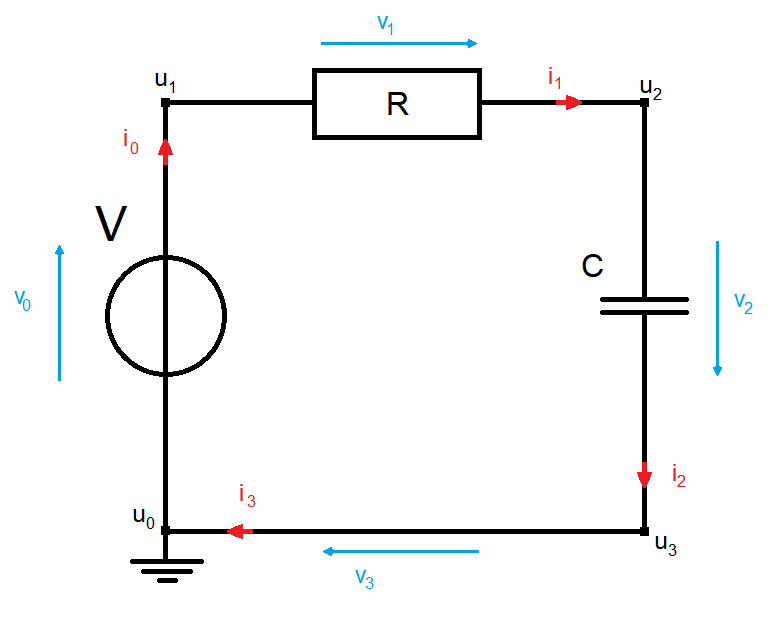
\includegraphics[scale=0.5]{pictures/Example1_simple.png}
		\caption{charging capacitor with series resistor and voltage source}
		\label{circuit:charging of capacitor}
	\end{figure}
	With the node-potentials, the voltages and the currents collected in the vectors
	\begin{displaymath}
		u=
		\left(
		\begin{matrix}
			u_0 \\
			u_1 \\
			u_2 \\
			u_3 
		\end{matrix}
		\right),
		\quad
		v=
		\left(
		\begin{matrix}
			v_0 \\
			v_1 \\
			v_2 \\
			v_3 
		\end{matrix}
		\right),
		\quad
		i=
		\left(
		\begin{matrix}
			i_0 \\
			i_1 \\
			i_2 \\
			i_3 
		\end{matrix}
		\right),
	\end{displaymath}
	the incidence matrix of this circuit has the form
	\begin{displaymath}
		\tilde{A} = 
		\left(
		\begin{matrix}
			1 & 0 & 0 & -1 \\
			-1 & 1 & 0 & 0 \\
			0 & -1 & 1 & 0 \\
			0 & 0 & -1 & 1 
		\end{matrix}
		\right).
	\end{displaymath}
	The rows of this matric correspond to the nodes of the circuit and the columns correspond to the edges and tell us if the edge either starts ($1$) or end ($-1$) at a node. By grounding node $u_0$ this matrix reduces to
	\begin{displaymath}
		A = 
		\left(
		\begin{matrix}
			-1 & 1 & 0 & 0 \\
			0 & -1 & 1 & 0 \\
			0 & 0 & -1 & 1 
		\end{matrix}
		\right).
	\end{displaymath}
	In this circuit edge 3 is not populated with any components. This means that the voltage along this edge does not change, or in terms of potentials
	\begin{displaymath}
		u_0 - u_3 = 0.
	\end{displaymath}
	Thus we can consider this circuit with node 0 and node 3 merged. This leads to a slightly different incidence and reduced incidence matrix, i.e.
	\begin{displaymath}
		\tilde{A} = 
		\left(
		\begin{matrix}
			1 & 0 & -1 \\
			-1 & 1 & 0 \\
			0 & -1 & 1 \\
		\end{matrix}
		\right) \quad \text{and} \quad
		A = 
		\left(
		\begin{matrix}
			-1 & 1 & 0 \\
			0 & -1 & 1 
		\end{matrix}
		\right), \quad \text{respectively.}
	\end{displaymath}
\end{example1}

\begin{example2}[LC-Circuit]
	\label{ex:LC-circuit incidence matrix}
	Our second example is a circuit that only contains a capacitor and an inductor, see Figure \ref{circuit:LC-circuit}. This circuit will oscillate, if given appropriate initial conditions.
	\begin{figure}[H]
		\centering
		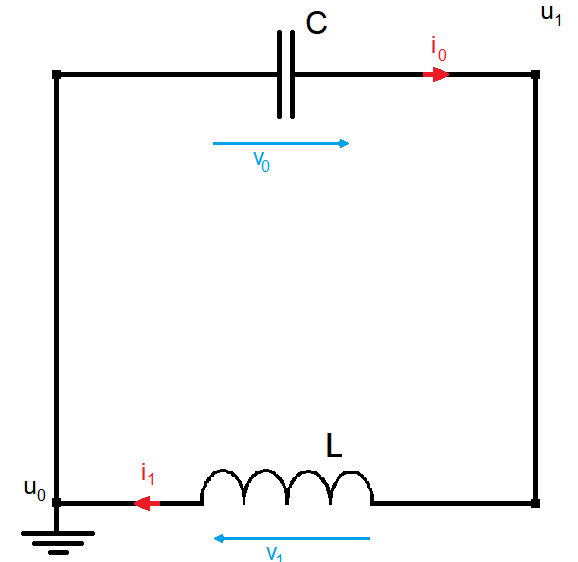
\includegraphics[scale=0.5]{pictures/Example2_index0.png}
		\caption{capacitor and inductor oscillator}
		\label{circuit:LC-circuit}
	\end{figure}
	
	We again collect the node-potentials, the voltages and the currents in the vectors
	\begin{displaymath}
		u=
		\left(
		\begin{matrix}
			u_0 \\
			u_1
		\end{matrix}
		\right),
		\quad
		v=
		\left(
		\begin{matrix}
			v_0 \\
			v_1
		\end{matrix}
		\right),
		\quad
		i=
		\left(
		\begin{matrix}
			i_0 \\
			i_1
		\end{matrix}
		\right).
	\end{displaymath}
	The incidence matrix of this circuit has the form
	\begin{displaymath}
		\tilde{A} = 
		\left(
		\begin{matrix}
			1 & -1  \\
			-1 & 1 
		\end{matrix}
		\right).
	\end{displaymath}
	By grounding node $u_0$ this can again be reduced, we obtain the reduced incidence matrix
	\begin{displaymath}
		A = 
		\left(
		\begin{matrix}
			-1 & 1  
		\end{matrix}
		\right).
	\end{displaymath}
\end{example2}

\begin{example3}[Parallel Voltage Source, Capacitor and Resistor]
	\label{ex:Example 3 - incidence matrix }
	As a third example we consider a similar circuit to the circuit presented in Example 1.\ref{ex:network topology}, the only difference is that we connected the resistor parallel to the capacitor instead of connecting it in series.
	\begin{figure}[H]
		\label{circuit:Example 3}
		\centering
		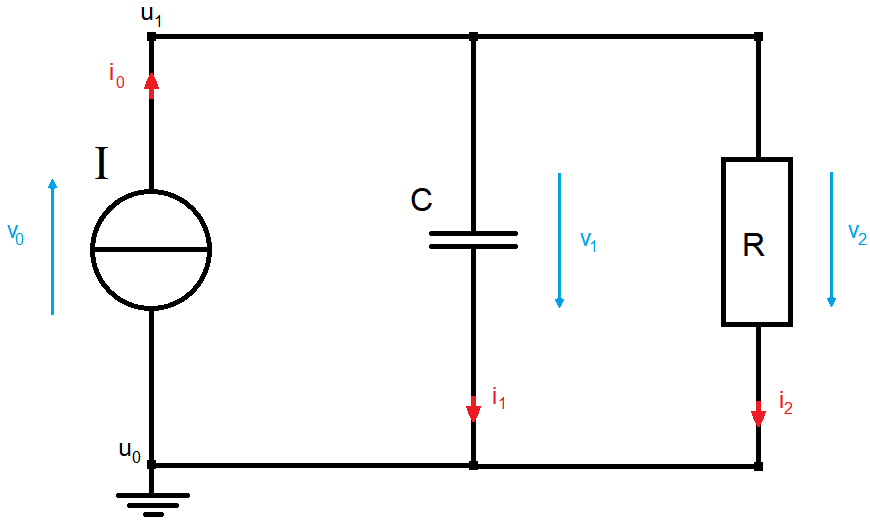
\includegraphics[scale=0.5]{pictures/Example3.png}
		\caption{Capacitor with resistor and voltage source}
	\end{figure}
	
	We collect the node-potentials, the voltages and the currents in the vectors
	\begin{displaymath}
		u=
		\left(
		\begin{matrix}
			u_0 \\
			u_1 
		\end{matrix}
		\right),
		\quad
		v=
		\left(
		\begin{matrix}
			v_0 \\
			v_1 \\
			v_2 
		\end{matrix}
		\right),
		\quad
		i=
		\left(
		\begin{matrix}
			i_0 \\
			i_1 \\
			i_2 
		\end{matrix}
		\right).
	\end{displaymath}
	The incidence matrix of this circuit has the form
		\begin{displaymath}
		\tilde{A} = 
		\left(
		\begin{matrix}
			1 & -1 & -1 \\
			-1 & 1 & 1 
		\end{matrix}
		\right),
	\end{displaymath}
	this leads to the reduced incidence matrix
	\begin{displaymath}
		A = 
		\left(
		\begin{matrix}
			-1 & 1 & 1
		\end{matrix}
		\right).
	\end{displaymath}
\end{example3}

\section{Energy Conservation Laws}
To fully fix all the variables that arise in the model of an electrical circuit we will need some \emph{conservation laws}. In this context, conservation laws are a description of physical properties that can be observed in electrical circuits. This means that they have to be fulfilled non-the-less, thus including them into the system also makes sense from a physical perspective. They were proposed by Kirchhoff in 1845, see \cite{KirchhoffsLaws}.
\begin{itemize}
	\item \textbf{Kirchhoff's voltage law (KVL):} \newline
	The sum of voltages along each loop of the network must equal to zero. Using the incidence matrix $A$ and the vector of potentials $u$ as well as the voltage vector $v$, this law can be formulated as
	\begin{equation}
		\label{KVL}
		A^\top  u = v.
	\end{equation}
	\item \textbf{Kirchhoff's current law (KCL):} \newline
	For any node, the sum of currents flowing into the node is equal to the sum of currents flowing out of the node. Using again the incidence matrix $A$ and the vector of currents $i$, this law can be formulated as
	\begin{equation}
		\label{KCL}
		A  i = 0.
	\end{equation}
\end{itemize}

\section{Electrical Components and their relations}
\label{Sec:Components relations}
Electrical components are described by equations relating their edge voltage $v$ to their edge current $i$. We will mainly focus on so-called RLC-networks (short for Resistor, Inductor and Capacitor). These networks consist only of resistors, capacitors, inductors, voltage sources and current sources. Diodes and transistors as well as other electrical components can be described in a similar way, although these lead to a more difficult analysis of the system, see e.g. \cite{ModellingAndDiscretizationOfCircuitProblems} and \cite{SchwarzTischendorfCircuitMNA}. Using the notation introduced in Section \ref{Sec:Network Topology}, the relations read as:
\begin{itemize}
	\item \textbf{Resistor} \newline
	Resistors ''resist`` the flow of current, which causes voltage to drop. This behaviour is described by the \emph{resistance} $R \in \mathbb{R}^+ := \{x \in \mathbb{R}: x > 0\}$ which is given in \emph{Ohm} ($\Omega$) and its reciprocal, the \emph{conductance} $G \in \mathbb{R}^+$, which is given in \emph{Siemens} ($S=\frac{1}{\Omega}$). 
	\begin{equation}
		\label{eq:resistor law}
		v = R \ i \quad \text{or} \quad i = G \ u.
	\end{equation}
	The electrical schematic symbol for resistors is depicted in Figure \ref{fig:resistor symbol}.
	\begin{figure}[H]
		\label{fig:resistor symbol}
		\centering
		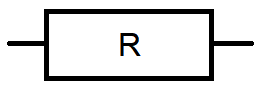
\includegraphics[width=2cm]{pictures/resistor.png}
		\caption{resistor symbol}
	\end{figure}

	\item \textbf{Capacitor} \newline
	Capacitors ''store`` electrical energy by accumulating electrical charge. Their characteristic equations can be described directly using the stored charge $Q \in \mathbb{R}^+_0 := \{x \in \mathbb{R}: x \geq 0\}$ or indirectly using the change in charge, which is nothing other than the current $I$. The \emph{capacitance} $C \in \mathbb{R}^+$ is given in \emph{Farads} ($F$).
	\begin{equation}
		\label{eq:capacitor law}
		Q = C \ v \quad \text{and by derivation in t} \quad I = \frac{d}{dt}Q = C \ \frac{d}{dt}v = C \ v'.
	\end{equation}
	The electrical schematic symbol for capacitors is depicted in Figure \ref{fig:capacitor symbol}.
	\begin{figure}[H]
		\label{fig:capacitor symbol}
		\centering
		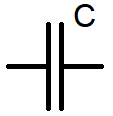
\includegraphics[width=2cm]{pictures/capacitor.png}
		\caption{capacitor symbol}
	\end{figure}

	\item \textbf{Inductor} \newline
	An electric current flowing through a conductor generates a magnetic field $\Phi \in \mathbb{R}^{n \times n}$ surrounding it. This magnetic field causes a voltage drop dependent on the change in current. The \emph{inductance} $L \in \mathbb{R}^+$ is given in \emph{Henry} ($H$).
	\begin{equation}
		\label{eq:inductor law}
		\Phi = L \ i \quad \text{and by derivation in t} \quad v = \Phi' = L \ i'.
	\end{equation}
	The electrical schematic symbol for inductors is depicted in Figure \ref{fig:inductor symbol}.
	\begin{figure}[H]
		\label{fig:inductor symbol}
		\centering
		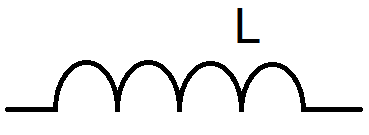
\includegraphics[width=3cm]{pictures/inductance.png}
		\caption{inductor symbol}
	\end{figure}

	\item \textbf{Voltage Source} \newline
	A voltage source supplies the system with a voltage. It can either supply varying amounts of voltage (with the special case of alternating current AC) or a fixed amount of voltage. The unit of voltage is \emph{Volts} ($V$).
	\begin{equation}
		\label{eq:voltage source law}
		v = v_{src}
	\end{equation}
	The electrical schematic symbol for voltage sources is depicted in Figure \ref{fig:voltage source symbol}.
	\begin{figure}[H]
		\label{fig:voltage source symbol}
		\centering
		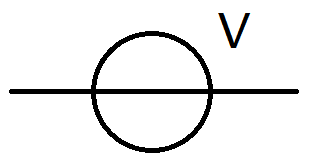
\includegraphics[width=4cm]{pictures/voltage_source.png}
		\caption{voltage source symbol}
	\end{figure}

	\item \textbf{Current Source} \newline
	A current source supplies the system with electrical current. It can either supply varying amounts of current (with the special case of alternating current AC) or a fixed amount of current. The unit of current is \emph{Ampere} ($A$).
	\begin{equation}
		\label{eq:current source law}
		i = i_{src}
	\end{equation}
	The electrical schematic symbol for current sources is depicted in Figure \ref{fig:current source symbol}.
	\begin{figure}[H]
		\label{fig:current source symbol}
		\centering
		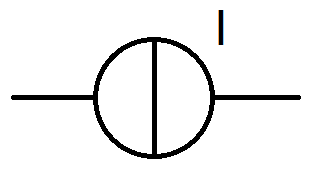
\includegraphics[width=4cm]{pictures/current_source.png}
		\caption{current source symbol}
	\end{figure}
	%\item Diode - to be filled with information after the rest is complete
	%\item Transistor - unlike the other components which were all two-teminal components a transisstor is a three-terminal component
\end{itemize}

The resistance $R$, conductance $G$, capacitance $C$ and inductance $L$ are respectively described as a scalar constant that relates the edge-current to the edge-voltage. If there are more components of the same kind in one circuit their corresponding constants will usually be collected into a matrix which is also called the same and also denoted by the same letter, respectively. These matrices are then positive definite diagonal matrices.

\section{Modified Nodal Analysis - MNA}
\label{sec:MNA}

%num gew dgl steif n steif - seite 422 \newline
%modelling discr circ prob - seite 19

\cite{ModellingAndDiscretizationOfCircuitProblems} and \cite{NumerikGewöhnlicherDifferentialgleichungen}

To analyse the network further we will rearrange the columns of the reduced incidence matrix $A$ such that it has the block form
\begin{displaymath}
	A = 
	\begin{pmatrix}
		A_R & A_C & A_L & A_V & A_I
	\end{pmatrix}
\end{displaymath}
where $A_R$, $A_C$, $A_L$, $A_V$ and $A_I$ include the columns that are related to the resistors, capacitors, coils, voltage sources and current sources, respectively.

To mathematically describe the circuit, we use \emph{modified nodal analysis} (or short MNA), see the paper by Ho, Ruehli and Brennan, \cite{MNA75}. MNA uses the node voltages as well as the currents of the coils and the voltage sources as unknowns. It is based on the conservation laws \eqref{KCL} and \eqref{KVL} as well as on the voltage-current relations of the electrical components, discussed in Section \ref{Sec:Components relations}. The voltages can be represented using the node-potentials and the incidence matrix $A$, i.e.
\begin{displaymath}
	v = A^\top u.
\end{displaymath}
The vector $v$ can thus be rearranged into $v = (v_R, v_C, v_L, v_{src}, v_I)$. In a similar way we also rearrange the current vector into $i = (i_R, i_C, i_L, i_V, i_{src})$. Using the sorted incidence matrix blocks, we can rewrite the resistor current relation as
	\begin{displaymath}
		i_R = G \ v_R = G \ A_R^\top u.
	\end{displaymath}
Analogously, we rewrite the capacitor relation as
	\begin{displaymath}
		i_C = C \ v'_C = C \ A_C^\top u'.
	\end{displaymath}

From Kirchhoffs current law \eqref{KCL} we deduce that
\begin{displaymath}
	A_C i_C + A_R i_R + A_L i_L + A_V i_V = -A_I i_{src}.
\end{displaymath}

We plug in the component relations derived above and obtain
\begin{displaymath}
	A_C C A_C^\top u' + A_R G A_R^\top u + A_L i_L + A_V i_V = -A_I i_{src}.
 \end{displaymath}

Combining this with the component law for inductors \eqref{eq:inductor law} and the potential-voltage relation for voltage sources \eqref{eq:voltage source law} we finally get the MNA equations
\begin{displaymath}
	\begin{aligned}
		A_C C A_C^\top u' + A_R G A_R^\top u + A_L i_L + A_V i_V &= - A_I i_{src} , \\
		L i_L'	- A_L^\top u &= 0 , \\
		-A_V^\top u &=  -v_{src}.
	\end{aligned}	
\end{displaymath}

In matrix form these read
\begin{equation}
	\label{MNA_Matrixform}
	\begin{pmatrix}
		A_C C A_C^\top & 0 & 0 \\
		0 & L & 0 \\
		0 & 0 & 0
	\end{pmatrix}
	*
	\begin{pmatrix}
		u' \\
		i_L' \\
		i_V'
	\end{pmatrix}
	+
	\begin{pmatrix}
		A_R G A_R^\top & A_L & A_V \\
		-A_L^\top & 0 & 0 \\
		-A_V^\top & 0 & 0 
	\end{pmatrix}
	*
	\begin{pmatrix}
		u \\
		i_L \\
		i_V
	\end{pmatrix}
	=
	\begin{pmatrix}
		-A_I i_{src} \\
		0 \\
		-v_{src}
	\end{pmatrix} , 
\end{equation}
where the diagonal matrices $C$, $G$ and $L$ contain the capacities, conductivities and inductors, respectively.

The resulting systems are \emph{stiff} systems. This means that for their numserical solution special care has to be put into which methods are suitable for solving these systems in a stable manner. For analyzing nonlinear components, other formulations can be used, e.g. the charge flux oriented formulation, for details see \cite{ModellingAndDiscretizationOfCircuitProblems}.


\begin{example1}[Charging of a Capacitor]
	\label{ex:MNA}
	We again consider the charging of a capacitor. The circuit is again given as in Example 1.\ref{ex:network topology}, where we have already derived the reduced incidence matrix
	\begin{displaymath}
		A = 
		\left(
		\begin{matrix}
			-1 & 1 & 0 \\
			0 & -1 & 1 
		\end{matrix}
		\right).
	\end{displaymath} 
	This matrix can be split into the three submatrices $A_V$, $A_R$ and $A_C$ containing the columns of the matrix $A$. Because there are no inductors as well as no current sources resent, the matrices $A_L$ and $A_V$ are empty. The diagonal matrices containing the components constants are
	\begin{displaymath}
		C = (C), \qquad L = (), \qquad G = (\frac{1}{R}).
	\end{displaymath}
	Plugging this into the formula \eqref{MNA_Matrixform} we obtain the system
	\begin{equation}
		\label{eq:ex1 MNA}
		\begin{pmatrix}
			0 & 0 & 0 \\
			0 & C & 0 \\
			0 & 0 & 0
		\end{pmatrix}
		*
		\begin{pmatrix}
			u_1' \\
			u_2' \\
			i_0'
		\end{pmatrix}
		+
		\begin{pmatrix}
			\frac{1}{R} & -\frac{1}{R} & -1 \\
			-\frac{1}{R} & \frac{1}{R} & 0 \\
			1 & 0 & 0 
		\end{pmatrix}
		*
		\begin{pmatrix}
			u_1 \\
			u_2 \\
			i_0
		\end{pmatrix}
		=
		\begin{pmatrix}
			0 \\
			0 \\
			-v_{src}
		\end{pmatrix}.
	\end{equation}
	
	Note that because $L$ is empty, the system does not contain any related equations to inductances.
\end{example1}


\begin{example2}[LC-Circuit]
	\label{ex:LC-circuit MNA}
	Similarly we also derived the incidence Matrix for this system in Example 2.\ref{ex:LC-circuit incidence matrix}, i.e.
	\begin{displaymath}
		A = 
		\left(
		\begin{matrix}
			-1 & 1  
		\end{matrix}
		\right).
	\end{displaymath}
	
	This matrix can be split into the two submatrices $A_C$ and $A_L$ containing the columns of the matrix $A$. Because we do not have any resistors, voltage sources or current sources, the matrices $A_R$, $A_V$ and $A_I$ are empty. The diagonal matrices containing the components constants are
	\begin{displaymath}
		C = (C), \qquad L = (L), \qquad G=().
	\end{displaymath}
	Plugging this into the formula \eqref{MNA_Matrixform} we obtain the system
	\begin{displaymath}
		\begin{pmatrix}
			C & 0 \\
			0 & L 
		\end{pmatrix}
		*
		\begin{pmatrix}
			u_1' \\
			i_L'
		\end{pmatrix}
		+
		\begin{pmatrix}
			0 & 1 \\
			-1 & 0
		\end{pmatrix}
		*
		\begin{pmatrix}
			u_1 \\
			i_L
		\end{pmatrix}
		=
		\begin{pmatrix}
			0 \\
			0 
		\end{pmatrix}.
	\end{displaymath}
\end{example2}


\begin{example3}[Parallel Voltage Source, Capacitor and Resistor]
	\label{ex:Example 3 - MNA}
	We consider the circuit introduced in Example 3.\ref{ex:Example 3 - incidence matrix }, with the corresponding incidence matrix
	\begin{displaymath}
		A = 
		\left(
		\begin{matrix}
			-1 & 1 & 1
		\end{matrix}
		\right).
	\end{displaymath} 
	This matrix can be split into the three submatrices $A_I$, $A_R$ and $A_C$ containing the columns of the matrix $A$. As there are no inductors and no voltage sources present, the matrices $A_L$ and $A_V$ are empty. The diagonal matrices containing the components constants are
	\begin{displaymath}
		C = (C), \qquad L = (), \qquad G = (\frac{1}{R}).
	\end{displaymath}
	Plugging this into the formula \eqref{MNA_Matrixform} we obtain the system
	\begin{equation}
		\label{eq:ex3 MNA}
		\begin{pmatrix}
			C & 0 \\
			0 & 0 
		\end{pmatrix}
		*
		\begin{pmatrix}
			u_1' \\
			i_V'
		\end{pmatrix}
		+
		\begin{pmatrix}
			\frac{1}{R} & -1 \\
			1 & 0
		\end{pmatrix}
		*
		\begin{pmatrix}
			u_1 \\
			i_V
		\end{pmatrix}
		=
		\begin{pmatrix}
			0 \\
			-v_{src}
		\end{pmatrix}.
	\end{equation}
\end{example3}

%\section{Charge-Flux oriented formulation of MNA}
%\label{sec:charge flux oriented formulation}
% This time we derive the charge and flux based formulations. We again use the KCL \eqref{KCL} and the component equations to formulate a system of equations. This means that instead of directly using current and voltage, we instead use the flux of the magnetic field \eqref{eq:inductor law} and the charge \eqref{eq:capacitor law}. We then obtain
%
%\begin{align}
%	A_C q' + A_R r(A_R^\top u,t) + A_L i_L + A_V i_V + A_I i(A^\top u, q', i_L, i_V, t) &= 0, \label{charge/flux-1} \\
%	\phi' - A_L^\top u &= 0, \label{charge/flux-2} \\
%	v(A^\top u, q', i_L, i_V, t) - A_V^\top u &= 0, \label{charge/flux-3} \\
%	q - q_C(A_C^\top u) &= 0, \label{charge/flux-4} \\
%	\phi - \phi_L(i_L) &= 0.  \label{charge/flux-5} 
%\end{align}
%
%Using node potentials $u$, branch currents through voltage and flux controlled elements $i_V$ and $i_L$, charges and fluxes $q$ and $\phi$, voltage dependent resistors $r$, voltage and current dependent charge and flux sources $q_C$ and $\phi_L$, controlled current and voltage sources $i_{src}$ and $v_{src}$.
%
%We call this formulation the \emph{charge-flux oriented modified nodal analysis}.
%
%%so it makes sense to use the conventional approach of MNA - compare with phd thesis 

\chapter{Differential Algebraic Equations}

von \cite{NumerikGewöhnlicherDifferentialgleichungen} und DAE lecture

The resulting MNA of electrical circuits leads to a special form of differential equations, namely \emph{differential algebraic equations} (DAE). Additionally to differential equations they also contain algebraic equations or are equivalent to such a system. They are distinct from ordinary differential equations in that the Jacobian matrix for a DAE system is singular. 
To understand the general solvability of those systems and to find good numerical methods we first have to take a look at the theory of such DAEs.

In the most general form a DAE can be written as:
Find $y:\mathbb{R} \to \mathbb{R}^n$ such that
\begin{equation}
	\label{Abstract_DAE}
	F(t, y(t), y'(t)) = 0, \qquad \forall t \in I
\end{equation}

with $F:\mathbb{R} \times \mathbb{R}^n \times \mathbb{R}^n \to \mathbb{R}^n$ sufficiently smooth and $I$ the time-interval. As this is usually too general, one has to consider more specific types of DAEs.
This chapter focuses on giving a brief overview of the different types of differential algebraic equations. We will discuss the specific form of linear systems with constant coefficients in more detail, as those are the systems that arise from modified nodal analysis of a RLC-system. Additionally this chapter also discusses the notion of the index of an MNA-system.

\section{Types of DAEs}

	Let us consider the following three types of DAEs.
	
	\begin{itemize}
		\item \textbf{Linear systems with constant coeffiecients} \newline
		are systems of the form: find $y$ such that
		\begin{equation}
			\label{DAE-const-coeff}
			A y'(t) + B y(t) = f(t) ,
		\end{equation}
		with $A,B \in \mathbb{R}^{n \times n}$, $A$ singular, $B$ regular and $f:\mathbb{R} \to \mathbb{R}^n$ a function in time. If $A$ is regular this equation can be transformed into an ordinary differental equation, since
		\begin{displaymath}
			y'(t) + A^{-1}By(t) = A^{-1} f(t)
		\end{displaymath}
		
		Thus it is reasonable to assume $A$ singular.
		
		\item \textbf{Linear time dependent systems}
		are systems of the form: find $y$ such that
		\begin{displaymath}
			A(t) y'(t) + B(t) y(t) = f(t) ,
		\end{displaymath}
		with $A, B:\mathbb{R} \to \mathbb{R}^{n \times n}$, $f:\mathbb{R} \to \mathbb{R}^n$ functions, such that for every $t \in \mathbb{R}$ the matrix $A(t)$ is singular and the matrix $B(t)$ regular.
		
		\item  \textbf{Structured (non-linear) systems} \newline
		are semi-explicit systems of the form: find $(y,z)$ such that
		\begin{align*}
			y'(t) &= f(t, y(t), z(t)) , \\
			0 &= g(t,y(t),z(t)) ,
		\end{align*}
		with $f:\mathbb{R} \to \mathbb{R}^n$ and $g:\mathbb{R} \to \mathbb{R}^d$ functions.
	\end{itemize}
	
	For our analysis of electrical networks, we will focus on linear systems with constant coefficients \eqref{DAE-const-coeff}. The other systems could for example occur when we additionally consider time-dependent component relations e.g. temperature. 
	A splitting of the variable $y$ is usually common, where we differ between the \emph{differential variable} and the \emph{algebraic variable}. A differential variable in this sense is the part of $y$, whose derivatives also appear in the differential algebraic equation. The algebraic variable on the other hand only appears in algebraic equations.

\subsection{Weierstraß-Kronecker normal form}
\label{chap:Weierstraß-Kronecker Normalform}
%kapitel aus buch seite 399 num gew dgl steif, kapitel 13.2.2

To determine the solvability of a linear system with constant coefficients \eqref{DAE-const-coeff}, we first need to introduce a normal form for the system, the \emph{Weierstraß-Kronecker normal form}. This normal form is dependent on the family $\{A,B\} := \{ \mu A+B|\mu \in \mathbb{R} \}$, which is called the  \emph{matrix pencil} of the DAE.

\begin{definition}
	The matrix pencil $\{ A,B\}$ is called \emph{regular} if there exists some $c \in \mathbb{R}$, such that $(cA+B)$ is regular (i.e. $det(cA+B) \neq 0$), otherwise it is called singular.
\end{definition}

\begin{theorem}[Jordan normal form \protect{\cite[Theorem~13.2.1]{NumerikGewöhnlicherDifferentialgleichungen}}]
	For every matrix $Q \in \mathbb{R}^{n \times n}$ there exists a regular matrix $T \in \mathbb{C}^{n \times n}$, such that
	\begin{displaymath}
		T^{-1}QT = J = diag(J_1, ..., J_r) \quad \text{with} \quad J_i = 
		\left(
		\begin{matrix}
			\lambda_i & 1 & & 0 \\
			0 & \lambda_i & \ddots & \vdots \\
			& \ddots & \ddots & 1 \\
			0 & \hdots & 0 & \lambda_i
		\end{matrix}
		\right)
		\in \mathbb{C}^{m_i \times m_i}
	\end{displaymath} 
	and $n = m_1 + ... + m_r$.
\end{theorem}

The matrix $J$ is called Jordan normal form of $Q$, the matrices $J_i$ are called Jordan Blocks, where $\lambda_i$ are the corresponding eigenvalues of $Q$. The matrix $J$ is uniquely determined by $Q$ except for the arrangement of the diagonal blocks. If $Q$ posesses only real eigenvalues, then $T$ can also be choosen from the reals. \newline
In order to seperate the equation \eqref{DAE-const-coeff} into an algebraic and a differential part, we transform the matrices $A$ and $B$ according to the following theorem.
%aus buch seite 401
\begin{theorem}[\protect{\cite[Satz~13.2.2]{NumerikGewöhnlicherDifferentialgleichungen}}]
	\label{Kronecker-Normalform}
	Let $\{ A,B \}$ be a regular matrix pencil. There exist $P,Q \in \mathbb{C}^{n \times n}$ such that
	\begin{displaymath}
		PAQ = 
		\left(
		\begin{matrix}
			I_d & 0 \\
			0 & N 
		\end{matrix}
		\right), \quad
		PBQ = 
		\left(
		\begin{matrix}
			R & 0 \\
			0 & I_{n-d}
		\end{matrix}
		\right)
	\end{displaymath}

	where
	\begin{displaymath}
		N = diag(N_1, ..., N_r) \quad \text{with} \quad N_i = 
		\left(
		\begin{matrix}
			0 & 1 & & 0\\
			& \ddots &\ddots & \\
			& & & 0 & 1 \\
			0 & & & 0
		\end{matrix}
		\right)
		\in \mathbb{R}^{n_i \times n_i}
	\end{displaymath}
	and R has Jordan normal form. By $I_k$ we denote the identity matrix of size $k \times k$.
\end{theorem}

\begin{proof}
	Because $\{A,B\}$ is a regular matrix pencil, there exists $c \in \mathbb{R}$ such that $(cA+B)$ is regular. Set
	\begin{displaymath}
		\hat{A} := (cA+B)^{-1}A, \quad \hat{B} := (cA+B)^{-1}B.
	\end{displaymath}
	Considering 
	\begin{displaymath}
		(cA+B)^{-1}(cA+B) = I \implies (cA+B)^{-1}B+c(cA+B)^{-1}A = I ,
	\end{displaymath}
	we get that
	\begin{displaymath}
		\hat{B} = I-c \hat{A} .
	\end{displaymath}
	Let $J_ {\hat{A}}$ be the Jordan normal form of $\hat{A}$, this means that there exists a regular matrix $T_1$ such that
	\begin{displaymath}
		T_1^{-1}AT_1 = J_{\hat{A}} =
		\left(
		\begin{matrix}
			W & 0 \\
			0 & \tilde{N} 
		\end{matrix}
		\right) .
	\end{displaymath}
	The matrix $W$ contains the Jordan blocks with eigenvalues which are nonzero, the matrix $\tilde{N}$ contains the Jordan blocks with eigenvalues equal to zero, thus $\tilde{N}$ is \emph{nilpotent}.
	The Jordan normal form $J_{\hat{B}}$ of $\hat{B}$ is given by
	\begin{displaymath}
		T_1^{-1} \hat{B} T_1 = J_{\hat{B}} = 
		\left(
		\begin{matrix}
			I-cW & 0 \\
			0 & I-c\tilde{N}
		\end{matrix}
		\right) .
	\end{displaymath}
	The following two transformations will allow us to get the desired structure.
	First we will transform $J_{\hat{A}}$ with
	\begin{displaymath}
		T_2 :=
		\left(
		\begin{matrix}
			W & 0 \\
			0 & I-c\tilde{N}
		\end{matrix}
		\right)
	\end{displaymath}
	in
	\begin{displaymath}
		T_2^{-1}J_{\hat{A}} = 
		\left(
		\begin{matrix}
			I & 0 \\
			0 & (I-c\tilde{N})^{-1}\tilde{N}
		\end{matrix}
		\right)
	\end{displaymath}
	and $J_{\hat{B}}$ in
	\begin{displaymath}
		T_2^{-1}J_{\hat{B}} =
		\left(
		\begin{matrix}
			W^{-1}-cI & 0 \\
			0 & I
		\end{matrix}
		\right) .
	\end{displaymath}
	Let now $R$ be the Jordan normal form of $(W^{-1}-cI)$ and $N$ be the normal form of $(I-c\tilde{N})^{-1}\tilde{N}$, this means
	\begin{displaymath}
		T_W^{-1}(W^{-1}-cI)T_W = R \quad \text{and} \quad T_{\tilde{N}}^{-1}(I-c\tilde{N})^{-1}\tilde{N}T_{\tilde{N}} = N
	\end{displaymath}

	Considering this definition together with the Neumann series of $(I-c\tilde{N})^{-1}$ we obtain
	\begin{displaymath}
		\tilde{N} (I-c\tilde{N})^{-1} = \tilde{N} (c \sum_{i=0}^{\infty} \tilde{N}^i) = \tilde{N} (c \sum_{i=0}^{k-1} \tilde{N}^i) = c \sum_{i=0}^{k-1} \tilde{N}^{i+1} = (c \sum_{i=0}^{k-1} \tilde{N}^{i}) \tilde{N}
	\end{displaymath}
	where we used that $\tilde{N}$ is nilpotent with nilpotency index $k$. This shows that $\tilde{N}$ and $(I-c\tilde{N})^{-1}$ commute.
	
	From this we can conclude that
	\begin{displaymath}
		N^k = [T_{\tilde{N}}^{-1}(I-c\tilde{N})^{-1}\tilde{N}T_{\tilde{N}}]^k = T_{\tilde{N}}^{-1}[(I-c\tilde{N})^{-1}\tilde{N}]^kT_{\tilde{N}} = T_{\tilde{N}}^{-1}(I-c\tilde{N})^{-k}\underbrace{\tilde{N}^k}_{=0}T_{\tilde{N}} = 0
	\end{displaymath}
	
	We used the commutativity in the third step here. The nilpotent matrix $N$ thus also has the nilpotency index $k$. A transformation with
	\begin{displaymath}
		T_3 := 
		\left(
		\begin{matrix}
			T_W & 0 \\
			0 & T_{\tilde{N}}
		\end{matrix}
		\right)
	\end{displaymath}
	transforms $T_2^{-1}J_{\hat{A}}$ into the Jordan normal form
	\begin{displaymath}
		J_{\tilde{A}} := T_3^{-1}T_2^{-1}J_{\hat{A}}T_3 = T_3^{-1}T_2^{-1}T_1^{-1}\hat{A}T_1T_3 = 
		\left(
		\begin{matrix}
			I & 0 \\
			0 & N
		\end{matrix}
		\right)
	\end{displaymath}
	and $T_2^{-1}J_{\hat{B}}$ into
	\begin{displaymath}
		J_{\tilde{B}} := T_3^{-1}T_2^{-1}J_{\hat{B}}T_3 = T_3^{-1}T_2^{-1}T_1^{-1}\hat{B}T_1T_3 = 
		\left(
		\begin{matrix}
			R & 0 \\
			0 & I
		\end{matrix}
		\right) .
	\end{displaymath}
	Now set
	\begin{displaymath}
		P:= T_3^{-1}T_2^{-1}T_1^{-1}(cA+B)^{-1} \quad \text{and} \quad Q = T_1T_3
	\end{displaymath}
	to get the statement.
\end{proof}

Using the findings above we are able to transform the initial DAE \eqref{DAE-const-coeff} using the matrix $P$ from Theorem \ref{Kronecker-Normalform}. By multiplying with $P$ from the left, we obtain
\begin{displaymath}
	P A y'(t) + P B y(t) = P f(t) .
\end{displaymath}

Setting
\begin{displaymath}
	y(t) = Q
	\left(
	\begin{matrix}
		u(t) \\
		v(t)
	\end{matrix}  
	\right) 
	, \quad
	Pf(t) = 
	\left(
	\begin{matrix}
		s(t) \\
		q(t)
	\end{matrix}
	\right),
\end{displaymath}
with $u(t),s(t) : \mathbb{R} \to \mathbb{R}^d$ and $q(t),v(t) : \mathbb{R} \to \mathbb{R}^{n-d}$.

We get a system of the form
\begin{equation}
	\label{transformed-DAE-const-coeff}
	\begin{aligned}
		u'(t) + Ru(t) &= s(t), \\
		Nv'(t) + v(t) &= q(t),
	\end{aligned}
\end{equation}

where $PAQ = 
\left( 
\begin{matrix}
	I & \\
	 & N
\end{matrix} 
\right)$
and $PBQ = 
\left( 
\begin{matrix}
	R & \\
	 & I
\end{matrix} 
\right)$.

We call this system the\emph{ Weierstraß-Kronecker normal form} of the DAE. The first equation of \eqref{transformed-DAE-const-coeff} is a first order ordinary differential equation and posesses a unique solution $u(t)$ in $[t_0,t_l]$ for any initial values $u_0 \in \mathbb{R}^d$. Now let $q(t) \in C^{k-1}([t_0,t_l])$, where $C^{k-1}(I)$ denotes the space of all functions with domain $I$ that are $k-1$ times continuously differentiable. We differentiate the second equation in \eqref{transformed-DAE-const-coeff} and obtain
\begin{align}
	\notag
	v(t) &= q(t) - Nv'(t) = q(t) - N(\underbrace{q(t)-Nv'(t)}_{=v(t)})' = q-Nq'+N^2v'' \\ \notag
	&= q-Nq'+N^2(q-Nv')'' = q-Nq'+N^2q''-N^3v''' \\ \notag
	&\vdots \\ \notag
	&= q-Nq'+...+(-1)^{k-1}N^{k-1}\underbrace{\frac{d^k}{dt^k}q}_{:=q^{(k-1)}}+(-1) \underbrace{N^kv^{(k)}}_{=0}\\ 
	\label{solution-to-transformed-DAE-const-coeff-part2}
	&= \sum_{i=0}^{k-1} (-1)^iN^iq^{(i)}(t)
\end{align}

where $k$ is the nilpotency index of $N$. Hence we have an explicit  form of the solution of $v(t)$. The Kronecker index $k$ thus tells us how many differentiations are required to obtain an ordinary differential equation. Note that this way of splitting the DAE allows us to differ between algebraic and differential variables.

We can also give a general definition of a DAE in Weierstraß-Kronecker normal form.
\begin{definition}[\protecting{\cite[Definition~13.2.4]{NumerikGewöhnlicherDifferentialgleichungen}}]
	A linear differential equation \eqref{DAE-const-coeff} is said to be in Weierstraß-Kronecker normal form if
	\begin{displaymath}
		A = 
		\left(
		\begin{matrix}
			I & 0 \\
			0 & N
		\end{matrix}
		\right), \quad
		B = 
		\left(
		\begin{matrix}
			R & 0 \\
			0 & I
		\end{matrix}
		\right),
	\end{displaymath}
	where $N$ is a nilpotent Jordan-block matrix.
\end{definition}

\begin{definition}
	The nilpotency index $k$ of the matrix $N$ from the Weierstraß-Kronecker Normalform of a matrix pencil $\{A,B\}$ with $A$ singular is called the \emph{Kronecker index} of $\{A,B\}$, which we denote by $ind\{A,B\}$. Note that for $A$ regular we set $ind\{A,B\} = 0$.
\end{definition}

%lemma 13.2.1

\begin{lemma}
	\label{Lemma:indipendence of Kronecker index}
	The Kronecker-Index $ind\{A,B\}$ is independent of the choice of the matrices $P$ and $Q$.
\end{lemma}

\begin{proof}
	See Lemma 13.2.1 in \protect{\cite[\pno403]{NumerikGewöhnlicherDifferentialgleichungen}}.
\end{proof}

%\begin{figure}
%	\centering
%	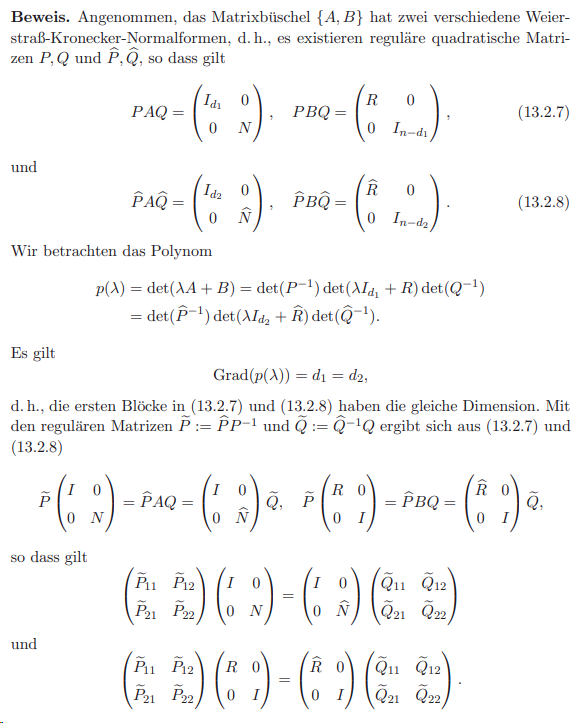
\includegraphics[width=0.7\linewidth]{screenshot003}
%	\caption{}
%	\label{fig:screenshot003}
%\end{figure}

%\begin{figure}
%	\centering
%	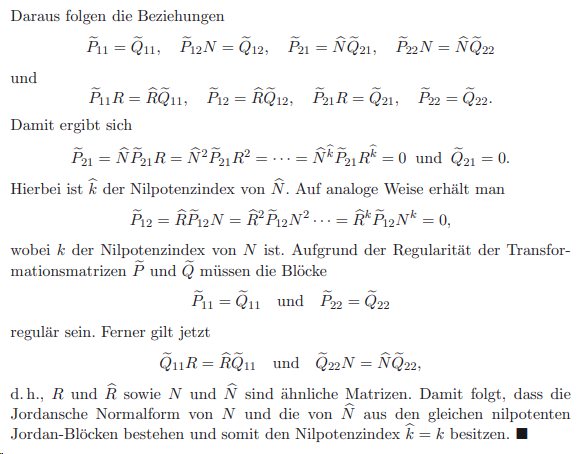
\includegraphics[width=0.7\linewidth]{screenshot004}
%	\caption{}
%	\label{fig:screenshot004}
%\end{figure}


%Lemma 13.2.2

\section{Index of a Differential Algebraic Equation}

The index of a DAE gives us insight about its numerical properties and in general about the solvability of the equation. In particular, as we will also mention later, the index is relevant for choosing initial values that allow us to solve the system uniquely.

We will consider two types of index concepts, the differentiation index and the perturbation index.

Since numerical differentiation is an unstable procedure the differentiation index aims to give a measure for the numerical problems to be expected when solving such systems.

\begin{definition}[Differentiation index \protect{\cite[Definition~13.3.1]{NumerikGewöhnlicherDifferentialgleichungen}}]
	Consider the differential algebraic equation \eqref{Abstract_DAE} to be uniquely locally solvable and $F$ sufficiently smooth. For a given $m \in \mathbb{N}$ consider the equations
	\begin{displaymath}
		\begin{aligned}
			F(t,y,y') &= 0, \\
			\diff{F(t,y,y')}{t} &= 0, \\
			&\vdotswithin{=} \\
			\diff[m]{F(t,y,y')}{t} &= 0.
		\end{aligned}
	\end{displaymath}
	The smallest natural number $m$ for which the above system results in an explicit system of ordinary differential equations (ODEs), i.e. it has the form
	\begin{displaymath}
		y' = \phi(t,y),
	\end{displaymath}
	is called \textbf{differentiation index}.
\end{definition}

In the previous chapter we have already discussed, that for a DAE with constant coefficients \eqref{DAE-const-coeff} and a regular matrix pencil $\{A,B\}$  we need $k = ind\{A,B\}$ differentiations to receive an ordinary differential equation. Hence for a DAE with constant coefficients the Kronecker index $k$ is equal to the differentiation index.

\begin{definition}[perturbation index \protect{\cite[Definition~13.3.3]{NumerikGewöhnlicherDifferentialgleichungen}}]
	Let $y(t)$ be the exact solution of \eqref{Abstract_DAE} and $\tilde{y}(t)$ be the solution of the perturbed system $F(t, \tilde{y}, \tilde{y}') = \delta(t)$. The smallest number $k \in \mathbb{N}$ such that 
	\begin{displaymath}
		\|y(t)-\tilde{y}(t)\| \leq C \left(\|y(t_0)-\tilde{y}(t_0)\|+\sum_{j=0}^{k}\max_{t_0 \leq \xi \leq T} \left\rVert 		\int_{t_0}^{\xi}\diff[j]{\delta}{\tau}(\tau)d \tau \right\rVert \right)
	\end{displaymath}
	for all $\tilde{y}(t)$, is called the \textbf{perturbation index} of this system.
\end{definition}	

We now consider the case of a perturbed linear DAE with constant coefficients and a regular matrix pencil $\{A,B\}$
\begin{displaymath}
	A \tilde{y}'(t) + B \tilde{y}(t) = -\delta(t).
\end{displaymath}

Then we obtain for the difference of the unperturbed system with the perturbed system 
\begin{displaymath}
	A(y'(t)-\tilde{y}'(t)) + B(y'(t)-\tilde{y}(t)) = \delta(t)
\end{displaymath}

Due to Theorem \ref{Kronecker-Normalform} we can transform this system into a system of the form \eqref{transformed-DAE-const-coeff} % (\textbf{how?} - bemerkung 13.3.5
\begin{align*}
	u'(t) - \tilde{u}'(t) + \hat{R} (u(t) - \tilde{u}(t) ) &= \delta_1(t), \\
	N(v'(t) - \tilde{v}'(t)) &= \delta_2(t),
\end{align*}

where $u(t)$ holds the first $d$ entries of $y(t):\mathbb{R} \to \mathbb{R}^n$ and $v(t)$ holds the remaining $n-d$ entries. According to \eqref{solution-to-transformed-DAE-const-coeff-part2}, the solution of the algebraic variable has the form
\begin{displaymath}
	v(t) - \tilde{v}(t) = \sum_{i=0}^{k-1} (-1)^iN^i \delta_2^{(i)}(t) 
\end{displaymath}

Thus the perturbation index is the same as the Kronecker-index $ind\{A,B\}$, see \cite{NumerikGewöhnlicherDifferentialgleichungen}. More over we observe that the error depends on the derivatives of the pertubation.

%might want to elaborate on that

%Another index concept is the so called \emph{tractability index}.  

\chapter{Index Analysis of the MNA}

der ane satz do + proof hopefully

seite 22 kap 7 netw top and dae ind for rlc - modelling and discretization circ prob

In the linear case, the capacitances, inductances and resistances are symmetrical positive definite (We consider them as matrices in this case). In the nonlinear case ... . Then it is called an RLC network.

In our further analysis we will only consider such RLC networks.

where the RLC components are described by linear functions with positive cap, res, ind- thus the matrices
\begin{displaymath}
	C:=\frac{\partial q_C(w)}{\partial w}, \quad L:=\frac{\partial \phi_L(w)}{\partial w}, \quad G:=\frac{\partial r(w)}{\partial w}
\end{displaymath}

are positive definite and symmetric.
generalized to ninlinear case we still need positive definiteness.


This means we consider the equations resulting from the analysis above. As a reminder, these equations are of the form \ref{DAE-const-coeff}

\begin{displaymath}
	A y'(t) + B y(t) = f(t).
\end{displaymath}

Specifically the obtained equations from the Modified Nodal Analysis \ref{MNA_Matrixform} are

\begin{displaymath}
	\begin{pmatrix}
		A_C C A_C^\top & 0 & 0 \\
		0 & L & 0 \\
		0 & 0 & 0
	\end{pmatrix}
	*
	\begin{pmatrix}
		\dot{u} \\
		\dot{i_L} \\
		\dot{i_V}
	\end{pmatrix}
	+
	\begin{pmatrix}
		A_R G A_R^\top & A_L & A_V \\
		-A_L^\top & 0 & 0 \\
		-A_V^\top & 0 & 0 ä
	\end{pmatrix}
	*
	\begin{pmatrix}
		u \\
		i_L \\
		i_V
	\end{pmatrix}
	=
	\begin{pmatrix}
		-A_I i_{src} \\
		0 \\
		-v_{src}
	\end{pmatrix}
\end{displaymath}

\section{General Index analysis}

Assuming the system only contains linear elements or is linearized at an operating point in order to investigate the system behaviour then the corresponding network equation represent a DAE with constant coefficients \ref{DAE-const-coeff}. We will denote $x=(u i_L i_V)^\top$.

\begin{itemize}
	\item \textbf{ODE-case}: \newline
	The matrix $B$ is regular in \ref{DAE-const-coeff}. This is the case if
	\begin{figure}[H]
		\centering
		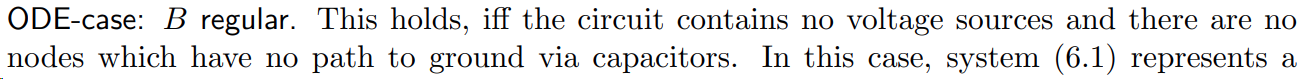
\includegraphics[width=0.7\linewidth]{screenshot006}
		\caption{}
		\label{fig:screenshot006}
	\end{figure}
	, then the system represents  a linear-implicit system of ODEs and can be transformed into the explicit ODE sytstem.
		
	\item \textbf{DAE-case}:
	The matrix $B$ is singular in \ref{DAE-const-coeff}. In the following we will assume $D$ to be regular. Multiplying with $D^{-1}$ from the left side produces
	\newline
	nevermind thats the same as we did in the \ref{DAE-const-coeff} chapter. - reference to that an explain in these terms. - page 20
\end{itemize}

The index of the MNA is the same as $ind(A,B)$, which denotes the nilpotency index of $N$ as we have seen in the previous analysis in chapter 3.


Investigating the index-cases further we can again distinct into two cases:

reminder for the structure obtained in previous chapter
\begin{align*}
	u'(t) + Ru(t) &= s(t), \\
	Nv'(t) + v(t) &= q(t)
\end{align*}

\begin{enumerate}
	\item index 1 case
	Because $N$ is nilpotent with nipotency index $\nu = 1$ it holds that $N^1 = 0$, thus the system transforms to
	\begin{align*}
		u'(t) + Ru(t) &= s(t), \\
		v(t) &= q(t).
	\end{align*}
	This means that the algebraic variables are given explicitly. Thus the system can be written in ODE form
	\begin{displaymath}
		\dot{x}=B^{-1}(-Ax+f(t)).
	\end{displaymath}

	\item index $\geq$ 2 case
	
	results in the solution we derived in \ref{solution-to-transformed-DAE-const-coeff-part2}.
\end{enumerate}

continue herer with modelling book from bottom of page 20-21

\section{Topological Conditions}
For this we consider RLC networks with independant voltage and current sources (\textbf{what does that mean?}). To obtain the perturbation index of the MNA we perturb the right-hand side of  
\newline reference to Tischendorf



basically chapter 7 of modelling book

From analyzing the MNA some conditions to the circuit topology can be obtained. We will be concidering the impact of loops containing only capacitances and voltage sources as well as cutsets containing only inductances and current sources.

In \cite{Tischendorf2005Topological} they present very interesting results about the index of MNA equations. Namely the following:


\begin{theorem}[Index-1 condition] \cite{Tischendorf2004Topological}
	Let the matrices of the capacitances, inductances and resistances respectively be positive definite. If the network neither cointains \emph{inductance-current-source cutsets} nor (controlled?) \emph{capacitance-voltage-source loops}, then the MNA leads to an index-1 DAE.
\end{theorem}

\begin{theorem}[Index-2 condition] \cite{Tischendorf2004Topological}
	If the Network contains \emph{inductance-current-source cutsets} or \emph{capacitance-voltage-source loops} except for capacitance-only loops, then the MNA leads to an index-2 DAE.
\end{theorem}

WE will apply those results to some examples:

\chapter{Numerical Solutions}
\label{sec:Numerical Solutions}

This chapter focuses on the numerical solution of the mentioned systems. It is based on results presented in \cite{NumerikGewöhnlicherDifferentialgleichungen} and \cite{HairerErnst1989Tnso}.

We will first focus on methods used to solve a more general initial value problem of the form:

Find y, such that
\begin{equation}
	\begin{aligned}
		y'(t) &= f(t,y), \quad t \in [t_0, t_l], \\
		y(t_0) &= y_0.
	\end{aligned}
	\label{general numerical problem}
\end{equation}

For this we presume that the function $f(t,y)$ is continuous and Lipschitz-continuous, we can apply the theorem of \emph{Picard-Lindelöf} \protecting{\cite[Satz~1.2.1]{NumerikGewöhnlicherDifferentialgleichungen}}, which states, that for every initial value $y_0$, the initial value problem \eqref{general numerical problem} is uniquely solvable in $[t_0, t_l]$.

In order to obtain an approximation to this unique solution we have to discretize. We first divide the time-intervall $[t_0, t_l]$ into smaller intervals
\begin{displaymath}
	I_{i+1} = [t_i, t_{i+1}] \quad \text{with} \quad i=0,...,N \text{ and } t_0 < t_1 < ... < t_N \leq t_l
\end{displaymath}

and consider approximations $y_m \approx y(t_m)$ on each interval $I_m$ with $m=1,...,N$, see Figure \ref{fig:numerical approximation} for an illustration. We call this a \emph{time-grid} and we call the difference $h_{ij} = t_j - t_i$ with $0 \leq i < j \leq N$ the \emph{step size} from $t_i$ to $t_j$. We will only consider equidistant grids, i.e. $h_{ij} = h$ for all $0 \leq i,j \leq N$. A function defined on such a grid is called a \emph{grid function}.

The grid function $y_h : T \to A$ with the time grid $T=\{t_0, ..., t_N\}$ and the approximated values $A = \{y_0, ..., y_N\}$ is called the \emph{numerical approximation} (of $y$ on the time grid).
\begin{figure}[H]
	\centering
	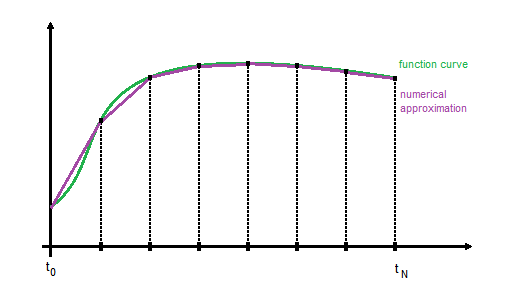
\includegraphics[scale=0.7]{pictures/num_approx.png}
	\caption{approximation of a function}
	\label{fig:numerical approximation}
\end{figure}

%\section{Single Step Methods}
%	The first class of numerical methods we will consider are single step methods. These methods use the previous approximated value $y_j$ and (for implicit methods) also the current approximated value $y_{j+1}$ to determine the current value $y_{j+1}$ through a \emph{procedural function}.
%	
%	\begin{definition}
%		\label{def:single step mehod}
%		A numerical method to approximate a differential equation \ref{general numerical problem} on a time-grid $T =\{t_0,...,t_l\}$ with the intermediate values $y_0,...,y_l$ is called a single step method, if it is of the form
%		\begin{equation}
%			\label{single-step method}
%			y_{j+1} = y_j + h_j \phi(t_j,y_j, y_{j+1},h_j).
%		\end{equation}
%		We call $\phi$ the \emph{procedural function}. If $\phi$ does not depend on $y_{j+1}$, then the method is called \emph{explicit}, otherwise it is called \emph{implicit}.
%	\end{definition}
%
%	\subsection{Consistency, Stability and Convergence}
%	
%	In order to compare different single-step methods we have to define the notions of consistency, stability and convergence. This leads to the definition of the error of the method, its consistency and its convergence. We begin with the definition of the error.
%	
%	\begin{definition}\label{Discretization_Error_SingleStep}
%		Let $y_{m+1}$ be the result of one step of a single step method \eqref{single-step method} with the exact start-vector $y_m = y(t_m)$ then
%		\begin{equation}
%			\label{local discretization error single step}
%			 \delta_{m+1} = \delta(t_m+h) = y(t_{m+1}) - \tilde{y}_{m+1}, \quad m = 0,...,N-1
%		\end{equation}
%		is called the \emph{local discretization error} of the single step method at the point $t_{m+1}$.
%	\end{definition}
%
%	The local error quantifies the error of every step of the method with respect to the exact solution. In most applications the exact solution is not known. Next we consider the consistency.
%
%	\begin{definition}\label{Consistency_SingleStep}
%		A single-step method is called \emph{consistent} if for all initial value problems \eqref{general numerical problem} 
%		\begin{equation}
%			\lim\limits_{h \to 0} \frac{\|\delta(t+h)\|}{h} = 0 \quad \text{for} \quad t_0 \leq t \leq t_l
%		\end{equation}
%		holds.\newline
%		It is called \emph{consistent of order p}, if for a sufficiently smooth function $f$
%		\begin{equation}
%			\|\delta(t+h)\| \leq Ch^{p+1} \quad \text{for all} \quad h \in \mathopen{(} 0,H \mathclose{]} \quad \text{and} \quad t_0 \leq t \leq t_l - h
%		\end{equation}
%		holds with $C$ independent of $h$.
%	\end{definition}
%
%	Consistency aims to give insight in how similar the problem \eqref{single-step method} that the numerical method solves is to the real problem \eqref{general numerical problem}. Finally we consider convergence of a single step method \ref{def:single step mehod}.
%
%	\begin{definition}\label{Convergence_SingleStep}
%		A single-step method is called \emph{convergent}, if for all initial value problems \eqref{general numerical problem} for the \emph{global discretization error}
%		\begin{displaymath}
%			e_m = y(t_m)-y_m
%		\end{displaymath}
%		holds that
%		\begin{displaymath}
%			\max\limits_{m}\|e_m\| \to 0 \quad \text{for} \quad h_{max} \to 0.
%		\end{displaymath}
%		The single-step method is called to have the \emph{convergence order} $p$, if
%		\begin{displaymath}
%			\max\limits_{m} \|e_m\| \leq C h_{max}^p \quad \text{for} \quad h_{max} \in \mathopen{(} 0,H \mathclose{]} \quad \text{with} \quad t_0 \leq t_m \leq t_l
%		\end{displaymath}
%		with the constant $C$ not dependent on the step size $h$.
%	\end{definition}
%
%	As the name suggestes convergence tries to quantify how far off a numerical solution is from the real solution of a system. A very interesting result follows if we additionally require the single-step method to be stable.
%	
%	\begin{definition}\label{Discrete_Stability_SingleStep - lecture notes for numpdgl}
%		A single-step method is called \emph{(discretely) stable} if for grid-functions $y_h$ and $\tilde{y}_h$ with
%		\begin{align}
%			y_{i+1} &= y_i + h \phi(t_i, y_i), \\
%			\tilde{y}_{i+1} &=  \tilde{y}_i + h [\phi(t_i, \tilde{y}_i) + \theta_i],
%		\end{align}
%		and perturbations $\theta_i = \theta_h(t_i)$ of the right side as well as a bounded perturbation in the initial-values $y_0 - \tilde{y}_0$ the error is bounded by
%		\begin{displaymath}
%			\|y_h - \tilde{y}_h\|_{\infty,h} \leq C (\|y_0 - \tilde{y}_0\|_{l^2} + \|\theta_h\|_{\infty,h})
%		\end{displaymath}
%		with a constant $C$ which is not dependent on $h$. The norm $\|.\|_{\infty,h}$ denotes the maximum norm over the time-grid, i.e. for a function $b: T={t_0,...,t_N} \to \mathbb{R}^d$ we have $\|b\|_{\infty,h} = \max\limits_{t \in T}\|b(t)\|$, $\|b\|$ is the euclidean norm.
%	\end{definition}
%	
%	For single-step methods which are consistent and stable we obtain the following convergence theorem.
%	
%	\begin{theorem}[Lax-Richtmyer]\label{Lax-Richtmyer}
%		A consistent (with order $p$) and discretely stable single-step method is convergent (with order $p$).
%	\end{theorem}
%	
%	This theorem is due to Lax and Richtmyer. The converse of this statement is also true. 
%
%	\subsection{Further stability properties}
%		from numpdgl skript \\
%		In this section we consider as a model problem the Dahlquist equation, i.e. find $y:\mathbb{R} \to \mathbb{C}$ such that
%		\begin{align}
%			y' &= \lambda y, \quad t > 0 \\
%			y(0) &= y_0
%		\end{align}
%		with $\lambda \in \mathbb{C}$ and $y_0 \in \mathbb{C}$ fixed.
%		
%		\begin{definition}
%			\begin{enumerate}
%				\item 
%				If a single-step method can be written in the form
%				\begin{equation}
%					y_{i+1} = R(z) \ y_i, \quad z:= h \lambda
%				\end{equation}
%				then we call $R: \mathbb{C} \to \mathbb{C}$ the \emph{stability function} of the single-step method.
%				\item 
%				The set
%				\begin{equation}
%					S := \{z \in \mathbb{C} : |R(z)| \leq 1\}
%				\end{equation}
%				is called the \emph{region of stability} of the method.
%				\item 
%				A single-step method is called
%				\begin{itemize}
%					\item \emph{0-stable}, if $0 \in S$.
%					\item \emph{A-stable}, if $\mathbb{C}^- \subset S$, where $\mathbb{C}^- = \{x \in \mathbb{C} : Re(x) \leq 0 \}$
%					\item \emph{L-stable}, if $R(z) \to 0$ for $Re(z) \to -\infty$.
%				\end{itemize}
%			\end{enumerate}
%		\end{definition}

	%\subsection{Runge-Kutta Methods}
	%	A very prevalent family of numerical single-step methods are the \emph{Runge-Kutta} methods. 
		
		%\begin{figure}
		%	\centering
		%	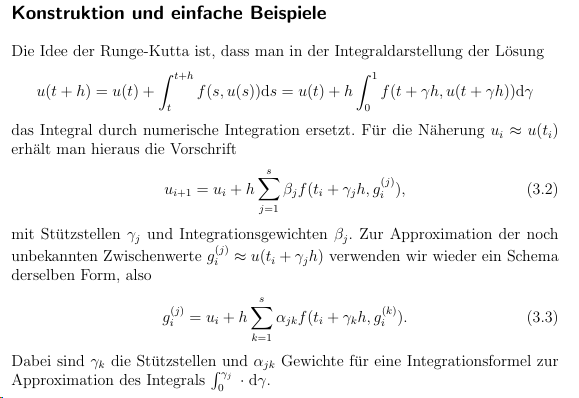
\includegraphics[width=0.7\linewidth]{screenshot026}
		%	\caption{}
		%	\label{fig:screenshot026}
		%\end{figure}
		
	%	\begin{definition}
	%		Let $s \in \mathbb{N}$. A single-step method of the form
	%		\begin{align}
	%			y_{m+1} = y_m + h \sum_{i=1}^{s} b_i f(t_m + c_ih, y_{m+1}^{(i)}) \\ 
	%			y_{m+1}^{(i)} = y_m +  \sum_{j=1}^{s} a_{ij} f(t_m + c_jh, y_{m+1}^{(j)})
	%		\end{align}
	%		is called a \emph{Runge-Kutta Method} with $s$ steps.
	%	\end{definition}
		
	%	We usually collect the coefficients into the vectors and matrices $c=(c_1, ...,c_s)$, $A = (a_{ij})_{ij}$ and $b=(b_1, ..., b_s)$.
		
	%	If $A$ is a strictly lower triangle matrix, this means for all $j \geq i$ holds $a_{ij} = 0$ then the Runge-Kutta method is explicit, otherwise it is implicit. In general implicit Runge-Kutta methods might need more computational effort because to calculate $y_m^{(i)}$ a nonlinear system of equations has to be solved. But in contrast those methods can also lead to very good stability characteristics.
		
	%	\begin{lemma}\cite{NumerikGewöhnlicherDifferentialgleichungen}
	%		A Runge-Kutta mehtod is consistent, if and only if
	%		\begin{displaymath}
	%			\sum_{i=1}^{s} b_i = 1
	%		\end{displaymath}
	%	\end{lemma}
	
	%	The coefficients of a Runge-Kutta method are usually represented in the \emph{Butchertableau}, which was introduced by John C. Butcher and has the following form.
		
	%	\begin{displaymath}
	%		\begin{array}{c|ccc}
	%			c_1 & a_{11} & \dots & a_{1s} \\
	%			\vdots & \vdots & & \vdots \\
	%			c_s & a_{s1} & \dots & a_{ss} \\
	%			\hline
	%			 & b_1 & \dots & b_s
	%		\end{array}
	%		\qquad
	%		\text{of in matrix form}
	%		\qquad
	%		\begin{array}{c|c}
	%			c & A \\
	%			\hline
	%			 & b
	%		\end{array}
	%	\end{displaymath}
	
	%	Their stability can directly be derived from the butcher tableau. The stability function of an arbitrary m-stage Runge-Kutta method has the form
	%	\begin{displaymath}
	%		R(z) = 1+zb^\top (I_m-zA)^{-1}e
	%	\end{displaymath}
	
	%	where $e = (1,...,1)$.
		
	%	\textbf{Remark:} The trapezoidal rule is a widely used Runge-Kutta method which we can also consider as a multistep-method. It will be discussed later on.
	
			
\section{Multistep Methods}
	\label{sec:multistep methods}
	
	In this thesis we will only consider the class of \emph{linear multistep methods} (LMSM). This chapter is in large parts based on \cite{NumerikGewöhnlicherDifferentialgleichungen}. These methods use multiple previously approximated values $y_{m+l}$ at the gridpooints  $t_{m+l}$, $l=0,1,...,k-1$ to approximate the current value $y_{m+k}$ at $t_{m+k}$. The definition for such a method is given in Definition \ref{def:multi step method}
	
	\begin{definition}
		\label{def:multi step method}
		For given $\alpha_0, ..., \alpha_k$ and $\beta_0, ..., \beta_k$ the iteration rule
		\begin{equation}
			\label{linear-multistep-method}
			\sum_{l=0}^{k} \alpha_l y_{m+l} = h \sum_{l=0}^{k} \beta_l f(t_{m+l}, y_{m+l}), \quad m=0,1,...,N-k
		\end{equation}
		is called a \emph{linear multistep method} (linear k-step method). It is always assumed that $\alpha_k \neq 0$ and $|\alpha_0| + |\beta_k| > 0$. If $\beta_k=0$ holds, then the method is called \emph{explicit}, otherwise it is called \emph{implicit}.
	\end{definition}
	
	The calculation of approximations using a multistep method consists of two phases:
	\begin{enumerate}
		\item In the \emph{starting-phase} approximations $y_1,...,y_{k-1}$ for the first $k-1$ gridpoints $t_l = t_0+l\ h, l=1,...,k-1$ have to be calculated. For example we can use a single-step method or a multi-step method with fewer steps.
		
		\item  In the \emph{run-phase} the multi-step formula is used to determine new approximations $u_{m+k}$ for the gridpoint $t_{m+k}$
	\end{enumerate}
	

	
	\subsection{Consistency, Stability and Convergence}
	
	In order to compare different multistep methods, we have to introduce the notions of error, consistency, stability and convergence. We begin with the definition of the error.
	\begin{definition}
		Let $y_{m+k}$ be the result of one step of the multi-step method \eqref{linear-multistep-method} with the start-values given as the evaluations of the exact solution $y_{m+l} = y(t_{m+l})$ at $0 \leq l < k$. This means
		\begin{displaymath}
			\alpha_k y_{m+k} = \sum_{l=0}^{k-1} \left( h \beta_l f(t_{m+l}, y(t_{m+l})) - \alpha_l y(t_{m+l}) \right) + h \beta_k f(t_{m+k}, y_{m+k}) .
		\end{displaymath}
		Then
		\begin{displaymath}
			\delta_{m+k} = y(t_{m+k}) - y_{m+k}, \quad m=0,1,...,N-k
		\end{displaymath}
		is called the \emph{local discretization error} (local error) of the linear multi-step method \eqref{linear-multistep-method} at the point $t_{m+k}$.
	\end{definition}
	
	If we assign the difference operator
	\begin{equation}
		L[y(t),h] = \sum_{l=0}^{k} \left( \alpha_l y(t+lh) - h \beta_l y'(t+lh) \right)
	\end{equation}
	to the linear mutli-step method, we gain the following definition for consistency of such a method.
	
	%%%%%%%%%%%%%%%%%%%%%%%%%%%%%%%%%%%%%%%%%%%%%%%%%%%%%%%%%%%%%%%pagebreak%%%%%%%%%%%%%%%%%%%%%%%%%%%%%%%%%%%%%%%%%%%%%%%%%%%%%%%%%%%%%%%%%%%%%%%%%%%%%%%%
	\newpage
	%%%%%%%%%%%%%%%%%%%%%%%%%%%%%%%%%%%%%%%%%%%%%%%%%%%%%%%%%%%%%%%%%%%%%%%%%%%%%%%%%%%%%%%%%%%%%%%%%%%%%%%%%%%%%%%%%%%%%%%%%%%%%%%%%%%%%%%%%%%%%%%%%%%%%%%%
	
	\begin{definition}
		A linear multi-step method is called %\emph{preconsistent} if for all functions $y(t) \in C^1[t_0,t_l]$
%		\begin{displaymath}
%			\lim\limits_{h \to 0} L[y(t),h]=0
%		\end{displaymath}
%		holds. 
%		It is called 
		\emph{consistent}, if for all functions $y(t) \in C^2([t_0,t_l])$
		\begin{displaymath}
			\lim\limits_{h \to 0} \frac{1}{h} L[y(t),h] = 0
		\end{displaymath}
		holds. It is called \emph{consistency with order p}, if for all functions $y(t) \in C^{p+1}[t_0, t_l]$
		\begin{displaymath}
			L[y(t),h] = \mathcal{O}(h^{p+1}) \quad \text{for} \quad h \to 0
		\end{displaymath}
		holds.
	\end{definition}

%	From the generating polynomials \eqref{eq:generating polynomials multistep method} we can derive simple consistency conditions, i.e.
%	\begin{displaymath}
%		\rho(1) = 0 \quad \text{and} \quad \rho'(1) = \sigma(1).
%	\end{displaymath}

	Next we introduce the convergence and the convergence order of such methods.
	
	\begin{definition} \label{def: LMSM convergence}
		We say that a linear multi-step method is convergent, if for a solution $y$ of the problem and a vector $(y_j)_{j=0}^k$ created by an LMSM , we have that
		\begin{displaymath}
			\lim\limits_{h \to \infty} \max_{0 \leq j \leq k} ||y(t_j) - y_j|| = 0.
		\end{displaymath}
		If for $p \in \mathbb{N}$ and a constant $C$ not dependent on the step size $h$ we have
		\begin{displaymath}
			\max_{0 \leq j \leq k} ||y(t_j) - y_j|| \leq Ch^p,
		\end{displaymath}
		then we call the LMSM \emph{convergent with order $p$}.
	\end{definition}
	
	%\begin{figure}
	%	\centering
	%	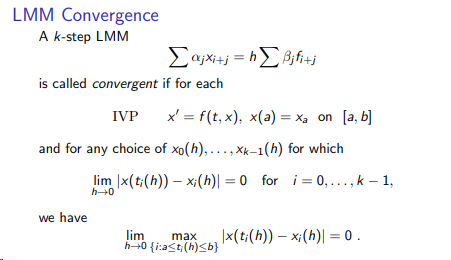
\includegraphics[width=0.7\linewidth]{screenshot025}
	%	\caption{}
	%	\label{fig:screenshot025}
	%\end{figure}
	
	The notion of stability tells us, if the output is continuously dependent on input. Thus we consider two different inputs for this definition and compare their outputs.
	
	%%%%%%%%%%%%%%%%%%%%%%%%%%%%%%%%%%%%%%%%%%%%%%%%%%%%%%%%%%%%%%%pagebreak%%%%%%%%%%%%%%%%%%%%%%%%%%%%%%%%%%%%%%%%%%%%%%%%%%%%%%%%%%%%%%%%%%%%%%%%%%%%%%%%
	\newpage
	%%%%%%%%%%%%%%%%%%%%%%%%%%%%%%%%%%%%%%%%%%%%%%%%%%%%%%%%%%%%%%%%%%%%%%%%%%%%%%%%%%%%%%%%%%%%%%%%%%%%%%%%%%%%%%%%%%%%%%%%%%%%%%%%%%%%%%%%%%%%%%%%%%%%%%%%
	
	\begin{definition} \label{discrete stability LMSM}
		A linear multi-step method is called (discretely) stable, if for solution vectors $(y_l)_{l=0}^k$ and $(\tilde{y}_l)_{l=0}^k$ of
		\begin{align}
			\sum_{l=0}^{k} \alpha_l y_{m+l} &= h \sum_{l=0}^{k} \beta_l f(t_{m+l}, y_{m+l}), \\
			\sum_{l=0}^{k} \alpha_l \tilde{y}_{m+l} &= h \sum_{l=0}^{k} \beta_l f(t_{m+l}, \tilde{y}_{m+l}) + h\theta_m,
		\end{align} 
		where and bounded initial values $y_j$, $\tilde{y}_j$ for $j \in {0,...,k}$, we have that
		\begin{displaymath}
			\max_{t_0 \leq t_n \leq T} ||y_n - \tilde{y}_n|| \leq C \sum_{j=0}^{k-1} ||y_j - \tilde{y}_j|| + \max_{t_0 \leq t_n \leq T} ||\theta_n||.
		\end{displaymath}
	\end{definition}
	
%	\begin{definition}
%		A linear multi-step method is called \emph{zero-stable} if all solutions of the difference equation
%		\begin{displaymath}
%			\sum_{l=0}^{k} \alpha_l u_{m+l} = 0
%		\end{displaymath}
%		are bounded.
%	\end{definition}
	
%	\textbf{Lax-Richtmyer}
	
%	\begin{theorem}
%		A linear multi-step method is zero-stable, if and only if the polynomial $\rho(x)$ fullfills the ``root-condition'', this means:
%		\begin{enumerate}
%			\item All roots $\bar{x}$ of $\rho(x)$ are within the unit-circle $|\bar{x}| \leq$ in the complex plane.
%			\item All roots $\bar{x}$ with $|x| = 1$ are singular.
%		\end{enumerate}
%	\end{theorem}
	
%	\begin{theorem}%[DAE lecture]
%		A linear multistep method is stable if and only if it is zero-stable.
%	\end{theorem}
	
	%\textbf{from circuit book below, above from modelling book}
	
	\subsection{Further stability properties}
	
	In this section we consider again the Dahlquist test problem as a model problem, i.e. find $y:\mathbb{R} \to \mathbb{C}$ such that
	\begin{align}
		y' &= \lambda y, \quad t > 0 \\
		y(0) &= y_0
	\end{align}
	with $\lambda \in \mathbb{C}$ and $y_0 \in \mathbb{C}$ fixed.\\
	
	%Asessment for stiff equations lt wikipedia (LMSM)
	
	Thus the resulting linear multistep method is of the form
	\begin{align*}
		\sum_{l=0}^{k} \alpha_l y_{n+l} = h \sum_{l=0}^{k} \beta_l \lambda y_{n+l} \\
		\iff \sum_{l=0}^{k}  [\alpha_l - h \beta_l \lambda] y_{n+l} = 0
	\end{align*}
	
	%in numerik book auf seite 326
	
	To be able to define further stability notions we first need to introduce the so called \emph{generating polynomials} of a multistep methods. They are defined using the coefficients of the method and thus hold a lot of information about the method. In the following we define these polynomials.
	\begin{equation}
		\label{eq:generating polynomials multistep method}
		\rho(x) := \sum_{l=0}^{k} \alpha_l x^l
		\qquad \text{and} \qquad
		\sigma(x) := \sum_{l=0}^{k} \beta_l x^l
	\end{equation}
	
	For the simpler class of mehthods called \emph{singlestep methods} there is a notion of A-stability, see \cite{NumerikGewöhnlicherDifferentialgleichungen}. Unfortunately for many multistep methods we do not have A-stability, thus we define the weaker $A(\alpha)$-stability.
	\begin{definition}
		\begin{enumerate}
			\item 
			The set
			\begin{equation}
				\begin{aligned}
					S := \{z \in \mathbb{C} : \rho(\xi) - z \sigma(\xi) = 0 \implies \xi \in \mathbb{C} \text{ and } |\xi| \leq 1. \\
					\text{ If $\xi$ has multiplicity greater than $1$, then } |\xi| < 1\}
				\end{aligned}
			\end{equation}
			is called the region of stability of the method.
			\item 
			A linear multistep method is called
			\begin{itemize}
				\item \emph{0-stable}, if $0 \in S$.
				\item stable in the point $z \in \mathbb{C}$, if $z \in S$.
				\item \emph{$A(\alpha)$-stable}, if it is stable in all $z$ that lie within the set $\{z \in \mathbb{C}^- : |arg(z)-\pi| \leq \alpha\}$ for $\alpha \in (0, \frac{\pi}{2})$.		 
			\end{itemize}
		\end{enumerate}
	\end{definition}
	
	%seite 314 im buch numerik 
	
	\begin{figure}[H]
		\centering
		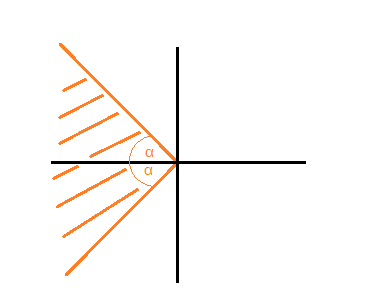
\includegraphics[width=0.3\linewidth]{pictures/A_alpha_stability.png}
		\caption{$A(\alpha)$ stability for $\alpha = \frac{\pi}{4}$}
		\label{fig:A of alpha stability}
	\end{figure}
	
	%following from numerik buch seite 134
	\begin{theorem}[\protecting{\cite[Satz~4.2.10]{NumerikGewöhnlicherDifferentialgleichungen}}]
		\label{th: null-stbaility and consistence is convergence}
		Let $f(t,y)$ be sufficiently smooth and the linear multi-step method be zero-stable and consistent of order $p$, then it is also convergent of order $p$.
	\end{theorem}
	
	%equivalent to lax richtmyer in single step because for lmsm zero stable = stable
	
\section{Implicit linear multistep formulas}
In this chapter we discuss three different linear multistep methods. Whereas the trapezoidal rule and the implicit midpoint rule (or Gauss with one stage) really only use one timestep to approximate the next value and might thus be considered as \emph{singlestep} methods, the Backward-Differentiation-Fomulas with $k$ stages (BDF-k) really use $k$ steps and thus are ``true'' multistep methods.
We will see that the BDF-k methods as well as the trapezoidal rule are preferably used over the implicit midpoint rule due to their advantageous behaviour when applied to differential algebraic equations. Examples are discussed in \ref{sec: numerical examples}. For more detailed analysis of the mentioned methods we refer to \cite{NumerikGewöhnlicherDifferentialgleichungen} and \cite{HairerErnst1989Tnso}.
%Our assumption that we only consider network equations arising from networks consisting of RLC components as well as controlled sources which keep the index between 1 and 2 still holds.

%We consider the equations in charge/flux oriented formulation introduced in section \ref{sec:charge flux oriented formulation}
%\begin{align*}
%	0 &=
%	\underbrace{ 
%	\left( \begin{matrix}
%		A_c & 0 \\
%		0 & I \\
%		0 & 0
%	\end{matrix} \right)}_{=:A}
%	\underbrace{
%	\left( \begin{matrix}
%		q' \\
%		\phi'
%	\end{matrix} \right)}_{=:y'}
%	+
%	\underbrace{
%	\left( \begin{matrix}
%		A_R r(A_R^\top u,t) + A_L i_L + A_V i_V + A_I i(u, i_L, i_V, t) \\
%		- A_L^\top u \\
%		v(u, i_L, i_V, t) - A_V^\top u
%	\end{matrix} \right)}_{=:f(x,t)}, \\
%	\underbrace{
%	\left( \begin{matrix}
%		q \\
%		\phi 
%	\end{matrix} \right)}_{=:y} 
%	&=
%	\underbrace{
%	\left( \begin{matrix}
%		q_C(A_C^\top u) \\
%		\phi_L(i_L) 
%	\end{matrix} \right)}_{=:g(x,t)},
%\end{align*}
%
%or simply
%\begin{align*}
%	0 &= F(y'(t), x(t), t) :=A y'(t) + f(x(t),t), \\
%	0 &= y(t) - g(x(t)).
%\end{align*}
%with the unknowns $x:=(u, i_L, i_V)^\top$.

In Section \ref{sec:multistep methods} we did already talk about the starting- and the run-phase of a multistep method. However, we left out one important aspect of the starting phase. Recall that in the starting phase we calculate the first $k-1$ steps using a method with fewer stages than the method we want to use ultimately. This also means that this method might be of lower order than the final method. To achieve the desired convergence rates it is thus also important to compute these initial steps appropriately, i.e. the method with which these initial steps are calculated has to also be of the desired order with respect to the \emph{final} step size $h$. (In applications this can mean that we calculate the initial steps with methods of lower order, but compensate by using a smaller step-size)

\subsection{BDF-k methods}
	\label{sec:BDFk}

	The Backward-Differentiation-Formulas with $k$ stages (or short \emph{BDF-k methods}) are constructed, such that they are $A(\alpha)$-stable with the largest possible angle $\alpha$. We will not go into detail about their construction, for this we again refer to \protecting{\cite[chapter~9.2]{NumerikGewöhnlicherDifferentialgleichungen}}

	We will not give a deeper look into their construction but will only state their properties. BDF schemes are appealing because they save function evaluations as much as possible.
	
	The BDF-k methods have the general form
	\begin{equation}
		\sum_{k=0}^{s} \alpha_k y_{n+k} = h \beta f(t_{n+s}, y_{n+s}).
	\end{equation}

	Due to the construction of the method, which is not built around conserving zero-stability, the method is not zero-stabel for all $k \in \mathbb{N}$. It turns out that it is only zero-stable for $k \leq 6$, \protecting{\cite[page~325]{NumerikGewöhnlicherDifferentialgleichungen}}. However in practice, methods with order greater than $3$ are rarely used because of their stability properties, as the stability-region shrinks with increasing order.
	
	The BDF or BDF-k formulas for $k=1,...,3$ have the following form %or till 6
	\begin{align*}
		k = 1 &: h f_{m+1} = y_{m+1} - y_m \\
		k = 2 &: h f_{m+2} = \frac{1}{2} (3 y_{m+2} - 4 y_{m+1} + y_m) \\
		k = 3 &: h f_{m+3} = \frac{1}{6} (11 y_{m+3} - 18 y_{m+2} + 9 y_{m+1} - 2 y_m) %\\
%		k = 4 &: h f_{m+4} = \frac{1}{12} (25 u_{m+4} - 48 u_{m+3} + 36 u_{m+2} - 16 u_{m+1} + 3 u_m) \\
%		k = 5 &: h f_{m+5} = \frac{1}{260} (137 u_{m+5} - 300 u_{m+4} + 300 u_{m+3} - 200 u_{m+2} +75 u_{m+1} -12 u_m) \\
%		k = 6 &: h f_{m+6} = \frac{1}{60} (147 u_{m+6} - 360 u_{m+5} + 450 u_{m+4} - 400 u_{m+3} + 225 u_{m+2} - 72 u_{m+1} + 10 u_m)
	\end{align*}
		
	As already mentioned BDF-k methods are not A-stable, but $A(\alpha)$ stable. In Figure \ref{fig:bdf-k stability regions} the stability regions for $k=1,2,3$ are depicted in cyan. Note that the zero-point is contained withing the stability regions.
		
	\begin{figure}[H]
		\centering
		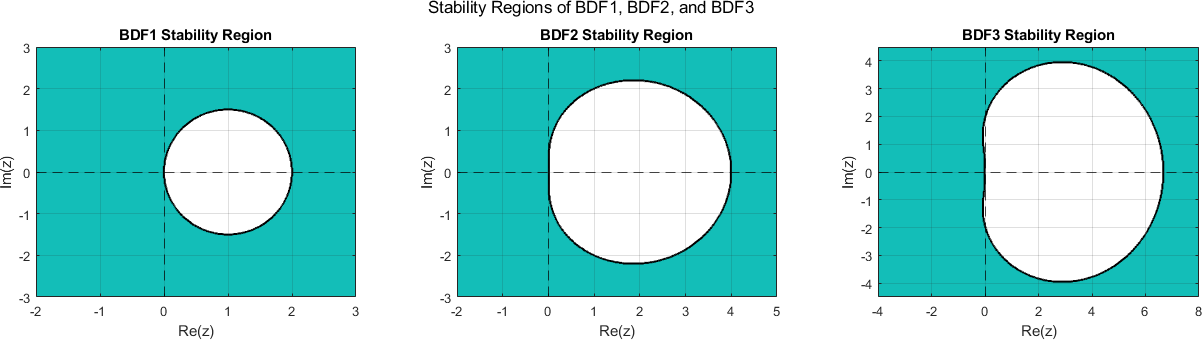
\includegraphics[width=1\linewidth]{pictures/bdf_stability_regions.png}
		\caption{stability regions of BDF-k methods for $k=1,2,3$ (cyan)}
		\label{fig:bdf-k stability regions}
	\end{figure}

	The order of consistency of this family of multi-step methods is given by the following theorem
	
	\begin{theorem}[\protecting{\cite[Satz~9.2.1]{NumerikGewöhnlicherDifferentialgleichungen}}]
		\label{th: BDK-k consistency}
		The BDF-k methods have consistency order $p=k$.
	\end{theorem}
	
	Due to Theorem \ref{th: null-stbaility and consistence is convergence} and the fact that BDF-k methods with $k \leq 6$  are $0$-stable as well as Theorem \ref{th: BDK-k consistency} we immediately gain the following corollary.
	
	\begin{corollary}[Convergence rate]
		The BDF-k methods with $k \leq 6$ are convergent with order$k$
	\end{corollary}
	
	%Seite 106 numerik - schrittweite für startwerte bei bdf3 kleiner für kleineren fehler, halbieren, vierteln, achteln whatever
	
\subsection{Trapezoidal rule}
	\label{sec:Trapezoidal}
	
	By approximating the area under a curve $f(x)$ on a short interval $[a,b]$ as a trapezoid, 
	\begin{displaymath}
		\int_{a}^{b} f(x) dx \approx (b-a)\frac{1}{2} (f(a)+f(b)),
	\end{displaymath}
	
	we can construct a numerical method for integrating a function. This method is called the trapezoidal rule, formally it has the iteration rule
	\begin{displaymath}
		y_{n+1} = y_n +\frac{h}{2}[f(t_n,y_n) + f(t_{n+1}, y_{n+1})].
	\end{displaymath}
	
	%	This iteration rule can also be formulated using the butcher tableau	
%	\begin{displaymath}
%		\begin{array}{c|cc}
%			0 & 0 & 0 \\
%			1 & \frac{1}{2} & \frac{1}{2} \\
%			\hline
%			& \frac{1}{2} & \frac{1}{2}
%		\end{array}
%	\end{displaymath}
	
	The trapezoidal rule has convergence order $p=2$ for our applications. For details see \cite{HairerErnst1989Tnso}, where more general the general form of the trapezoidal rule, namely the Lobatto~\RomanNumeralCaps{3}-A methods amongst other methods are discussed.
	
	Due to the fact that the trapezoidal rule is A-stabe  (\cite{ModellingAndDiscretizationOfCircuitProblems}) and of order $p=2$, it can be considered as a natural alternative to the BDF-2 method.
	
	%order p=2 because it is a special case of Lobatto 3 A with s=2, thus all the index cases just lead to p=2
	
\subsection{Gauss Method with one stage}
	\label{sec:Gauss1}

	We have already seen that the results for the BDF-k methods as well as for the trapezoidal rule are relatively straight forward. But this is not always the case, many numerical methods can cause problems when applied to DAEs, see also \cite{HairerErnst1989Tnso}. To illustrate this we will have a look at the Gauss method with one stages, also called the implicit midpoint rule, i.e.
	\begin{displaymath}
		y_{n+1} = y_n + h f(t_n + \frac{h}{2}, \frac{y_n + y_{n+1}}{2})
	\end{displaymath}

	Applied to ordinary differential equations, this method yields a convergence order of $p=2$ \protecting{\cite[chapter~8.1.2]{NumerikGewöhnlicherDifferentialgleichungen}}. For the special case of differential algebraic equations this does not hold true. Here we may observe lower convergence rates, especially in the algebraic variable. The convergence orders for this method are also different, if the amount of stages is even or odd. We say that this method is \emph{not stiffly accurate}. Table \ref{tab:convergence order Gauss} displays the according convergence orders.
	
	\begin{table}[H]
		\centering
		\begin{tabular}{ | c | c c | c c |}
			\hline
			\multirow{2}*{number of stages $s$} & \multicolumn{2}{c |}{index $\nu = 1$} & \multicolumn{2}{ c |}{index $\nu = 2$} \\
			 & differential & algebraic & differential & algebraic \\
			 \hline
			 even & \multirow{2}*{$2s$} & $s+1$ & $s+1$ & $s-1$ \\
			 odd & & $s$ & $s$ & $s-2$ \\
			 \hline
		\end{tabular}
		\caption{Convergence order for Gauss method.}
		\label{tab:convergence order Gauss}
	\end{table}
	
\section{Numerical Examples}
	
	\label{sec: numerical examples}
	In this section we will apply the trapezoidal rule, the BDF-k method and the implicit midpoint rule, discussed in Section \ref{sec:BDFk}, Section \ref{sec:Trapezoidal} and Section \ref{sec:Gauss1} to our three examples. We will also discuss the discretization error in the solution and compute appropriate consistant inital values for our problems. The code used is provided in Section \ref{sec:Code listings}.
	

\subsection{BDF-k Method and Trapezoidal Rule}	

	We will start by applying the ``well-behaving'' methods to our examples.
	
\begin{example1}[Numerical computation]
	We again consider the charging of a capacitor, depicted in the schematics in Figure \ref{fig:charging capacitor}.
	
	\begin{figure}[H]
		\centering
		\begin{minipage}{.5\textwidth}
			\centering
			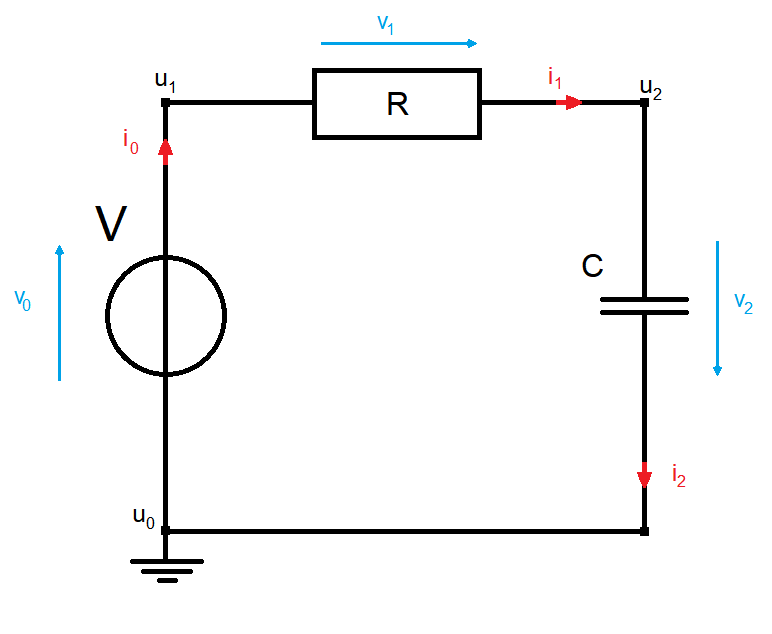
\includegraphics[width=\linewidth]{pictures/Example1_simple_p2.png}
			\caption{charging capacitor with series resistor and voltage source}
			\label{fig:charging capacitor}
		\end{minipage}%
		\begin{minipage}{.5\textwidth}
			\centering
			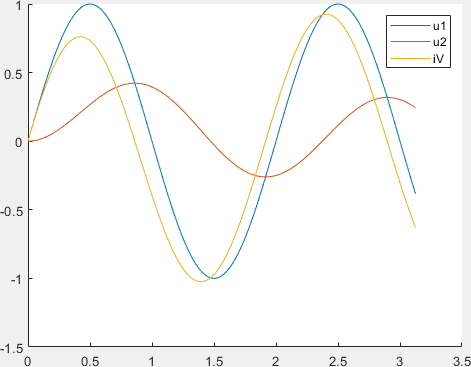
\includegraphics[width=\linewidth]{../Matlab/exact_solution_ex1.png}
			\caption{Exact solution for example 1.}
			\label{fig: Exact solution for example 1}
		\end{minipage}
	\end{figure}
	
	For testing we set the resistance to $R=1$ and the capacitance to $C=1$. In our case we let the  voltage source supply a voltage of the form $v_{src} = sin(\pi t)$. The resulting MNA-system for this example reads
	\begin{equation}
		\label{eq:MNA-system of chargin capacitor with explicit values}
		\begin{pmatrix}
			0 & 0 & 0 \\
			0 & 1 & 0 \\
			0 & 0 & 0
		\end{pmatrix}
		*
		\begin{pmatrix}
			u_,' \\
			u_2' \\
			i_0'
		\end{pmatrix}
		+
		\begin{pmatrix}
			1 & 1 & -1 \\
			1 & 1 & 0 \\
			1 & 0 & 0 
		\end{pmatrix}
		*
		\begin{pmatrix}
			u_1 \\
			u_2 \\
			i_0
		\end{pmatrix}
		=
		\begin{pmatrix}
			0 \\
			0 \\
			-sin(\pi t)
		\end{pmatrix}.
	\end{equation}
		
	We expect the resulting potentials and currents to be of the form seen in Figure \ref{fig: Exact solution for example 1}.

	The resulting errors for our numerical tests are displayed in table \ref{tab:num results ex1}, we omit $u_1$ since it just equals $-v_{src}$ and thus produces no interesting error results. The reported errors are computed using $err(y) = \max\limits_{0 \leq n \leq N} | y(t_n) - y_n |$ where $y_n$ denotes the numerical approximation and $y(t_n)$ denoted the exact solution at the time-step $t_n$. 
	
	\begin{table}[H]
		\resizebox*{\textwidth}{!}{%
			\csvreader[tabular= | c || c c | c c | c c | c c |,
			table head = \hline h & \multicolumn{2}{c|}{k = 1} & \multicolumn{2}{c|}{k = 2} & \multicolumn{2}{c|}{k = 3} & \multicolumn{2}{c|}{trapezoidal}\\
			& $err(u_2)$ & $err(i_V)$ & $err(u_2)$ & $err(i_V)$ & $err(u_2)$ & $err(i_V)$ & $err(u_2)$ & $err(i_V)$  \\
			\hline,
			late after line=\\\hline]
			{../Matlab/err_ex1.csv}{h=\h, oneu=\oneu, oneueoc=\oneueoc, oneuu=\oneuu, oneuueoc=\oneuueoc, onei=\onei, oneieoc=\oneieoc, twou=\twou, twoueoc=\twoueoc, twouu=\twouu, twouueoc=\twouueoc, twoi=\twoi, twoieoc=\twoieoc, threeu=\threeu, threeueoc=\threeueoc, threeuu=\threeuu, threeuueoc=\threeuueoc, threei=\threei, threeieoc=\threeieoc, trapu=\trapu, trapueoc=\trapueoc, trapuu=\trapuu, trapuueoc=\trapuueoc, trapil=\trapil, trapileoc=\trapileoc}
			{\h  & \num{\oneuu} & \num{\onei} & \num{\twouu} & \num{\twoi} & \num{\threeuu} & \num{\threei} & \num{\trapuu} & \num{\trapil}}
		}
		\caption{Resulting errors for the BDF-k methods and the trapezoidal rule.}
		\label{tab:num results ex1}
	\end{table}
	
%	\begin{table}[H]
%		\resizebox*{\textwidth}{!}{%
%			\csvreader[tabular= | c || c c c c | c c c c | c c c c | c c c c |,
%			table head = \hline h & \multicolumn{2}{c|}{k = 1} & \multicolumn{2}{c|}{k = 2} & \multicolumn{2}{c|}{k = 3} & \multicolumn{2}{c|}{trapezoidal}\\
%			& $err(u_2)$ & eoc & $err(i_V)$ & eoc & $err(u_2)$ & eoc & $err(i_V)$ & eoc & $err(u_2)$ & eoc & $err(i_V)$ & eoc & $err(u_2)$ & eoc & $err(i_V)$ & eoc \\
%			\hline,
%			late after line=\\\hline]
%			{../Matlab/err_ex1.csv}{h=\h, oneu=\oneu, oneueoc=\oneueoc, oneuu=\oneuu, oneuueoc=\oneuueoc, onei=\onei, oneieoc=\oneieoc, twou=\twou, twoueoc=\twoueoc, twouu=\twouu, twouueoc=\twouueoc, twoi=\twoi, twoieoc=\twoieoc, threeu=\threeu, threeueoc=\threeueoc, threeuu=\threeuu, threeuueoc=\threeuueoc, threei=\threei, threeieoc=\threeieoc, trapu=\trapu, trapueoc=\trapueoc, trapuu=\trapuu, trapuueoc=\trapuueoc, trapil=\trapil, trapileoc=\trapileoc}
%			{\h  & \num{\oneuu} & \num{\oneuueoc} & \num{\onei} & \num[exponent-mode=fixed,round-precision=2]{\oneieoc} & \num{\twouu} & \num{\twouueoc} & \num{\twoi} & \num{\twoieoc} & \num{\threeuu} & \num{\threeuueoc} & \num{\threei} & \num{\threeieoc} & \num{\trapuu} & \num{\trapuueoc} & \num{\trapil} & \num{\trapileoc}}
%		}
%		\caption{Resulting errors for the BDF-k methods and the trapezoidal rule.}
%		\label{tab:num results ex1}
%	\end{table}
	
	The errors presented in Table \ref{tab:num results ex1} confirm our results from Section \ref{sec:BDFk} and \ref{sec:Trapezoidal}, i.e. the BDF-k schemes have convergence order $p=k$ and the trapezoidal rule has convergence order $p=2$.
\end{example1}
		
	
\begin{example2}[Numerical computation]
	For this example we again consider the LC-circuit given in Figure \ref{fig: LC-circuit}.
	
	\begin{figure}[H]
		\centering
		\begin{minipage}{.5\textwidth}
			\centering
			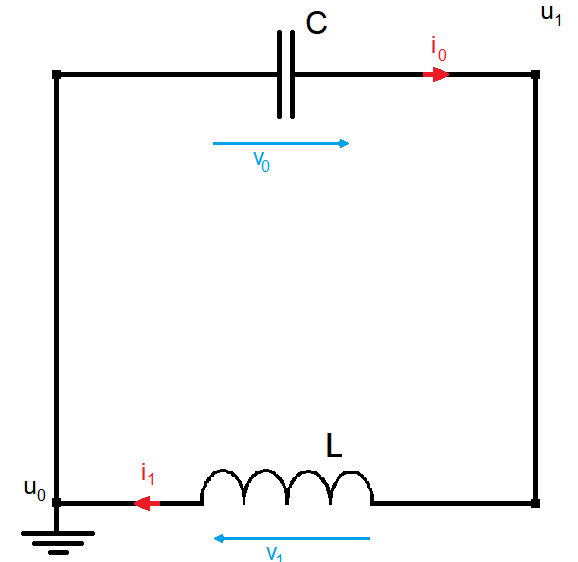
\includegraphics[width=\linewidth]{pictures/Example2_index0.png}
			\caption{LC-circuit}
			\label{fig: LC-circuit}
		\end{minipage}%
		\begin{minipage}{.5\textwidth}
			\centering
			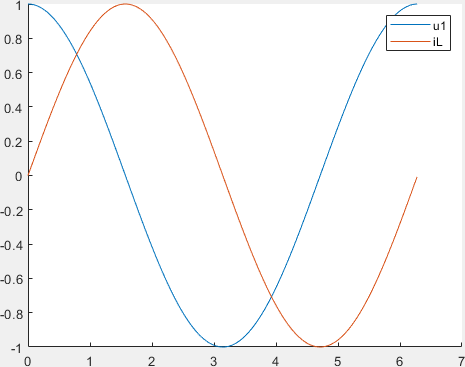
\includegraphics[width=\linewidth]{../Matlab/exact_solution_ex2.png}
			\caption{Exact solution for example 2.}
			\label{fig: Exact solution for example 2}
		\end{minipage}
	\end{figure}
	
	We again set $L=1$ and $C=1$. The resulting MNA-system for this example then reads
	
	\begin{displaymath}
		\begin{pmatrix}
			1 & 0 \\
			0 & 1 
		\end{pmatrix}
		*
		\begin{pmatrix}
			u_1' \\
			i_L'
		\end{pmatrix}
		+
		\begin{pmatrix}
			0 & 1 \\
			-1 & 0
		\end{pmatrix}
		*
		\begin{pmatrix}
			u_1 \\
			i_L
		\end{pmatrix}
		=
		\begin{pmatrix}
			0 \\
			0 
		\end{pmatrix}.
	\end{displaymath}
	
	When applying the BDF-k methods in Section \ref{sec:BDFk} and the trapezoidal rule in Section \ref{sec:Trapezoidal} to this problem, we can observe the maximal error $err(y) = \max\limits_{0 \leq n \leq N} | y(t_n) - y_n |$. The error is displayed in Table \ref{tab:error ex2}, where we again observe, that the errors reflect the predicted convergence rates.
		
	\begin{table}[H]
		\resizebox*{\textwidth}{!}{%
			\csvreader[tabular= | c || c c | c c | c c | c c | ,
			table head = \hline h & \multicolumn{2}{c|}{k = 1} & \multicolumn{2}{c|}{k = 2} & \multicolumn{2}{c|}{k = 3} & \multicolumn{2}{c|}{trapezoidal} \\
			& $err(u_1)$ & $err(i_l)$ & $err(u_1)$ & $err(i_l)$ & $err(u_1)$ & $err(i_l)$ & $err(u_1)$ & $err(i_l)$ \\
			\hline,
			late after line=\\\hline]
			{../Matlab/err_ex2.csv}{h=\h, oneu=\oneu, onei=\onei, twou=\twou, twoi=\twoi, threeu=\threeu, threei=\threei, trapu=\trapu, trapil=\trapil}
			{\h & \num{\oneu} & \num{\onei} & \num{\twou} & \num{\twoi} & \num{\threeu} & \num{\threei} & \num{\trapu} & \num{\trapil}}
		}
		\caption{Resulting errors for the BDF-k methods and the trapezoidal rule.}
		\label{tab:error ex2}
	\end{table}

\end{example2}
	


\begin{example3}[Numerical computation]
	
	In our last example we consider again the circuit given in Figure \ref{fig:num ex3}.
	\begin{figure}[H]
		\centering
		\begin{minipage}{.5\textwidth}
			\centering
			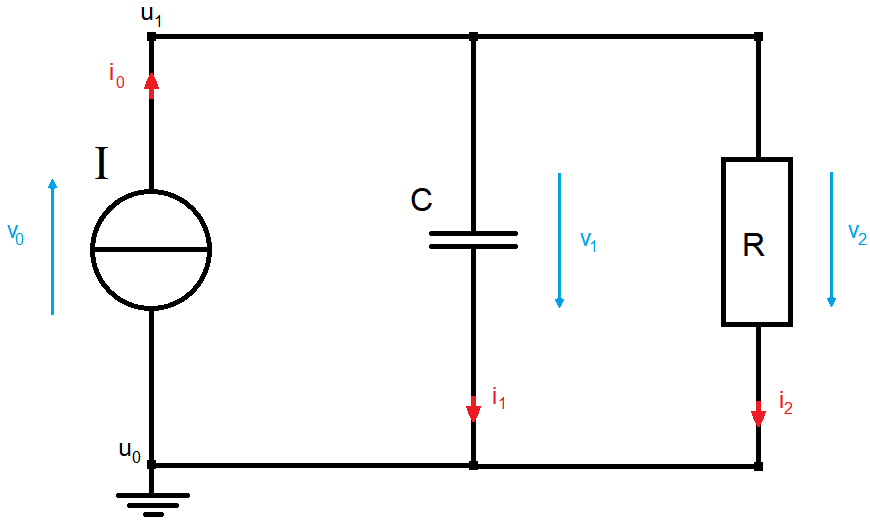
\includegraphics[width=\linewidth]{pictures/Example3.png}
			\caption{Current source with capacitor and resistor.}
			\label{fig:num ex3}
		\end{minipage}%
		\begin{minipage}{.5\textwidth}
			\centering
			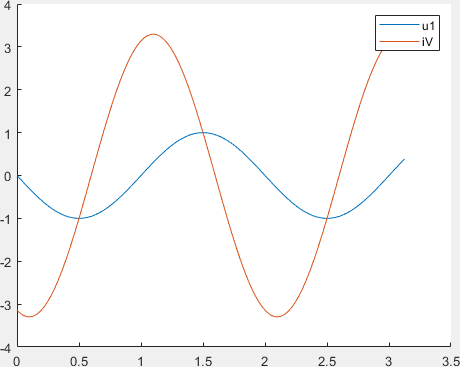
\includegraphics[width=\linewidth]{../Matlab/exact_solution_ex3.png}
			\caption{Exact solution for example 3.}
			\label{fig: Exact solution for example 3}
		\end{minipage}
	\end{figure}
	
	Setting $R=1$, $C=1$ and $v_{src} = sin(\pi t)$ the resulting system has the form
	\begin{displaymath}
			\begin{pmatrix}
			1 & 0 \\
			0 & 0 
		\end{pmatrix}
		*
		\begin{pmatrix}
			u_1' \\
			i_V'
		\end{pmatrix}
		+
		\begin{pmatrix}
			1 & -1 \\
			1 & 0
		\end{pmatrix}
		*
		\begin{pmatrix}
			u_1 \\
			i_V
		\end{pmatrix}
		=
		\begin{pmatrix}
			0 \\
			-sin(\pi t)
		\end{pmatrix}.
	\end{displaymath}
		
	With this we expect the potential and current to be given as illustrated in Figure \ref{fig: Exact solution for example 3}.

	The numerical methods result in errors displayed in Table \ref{tab:error ex3}. Due to the fact, that $u_1$ is again the same as $-v_{src}$, it is not of interest for our comparison of the errors, hence we omit $u_1$.
	
	\begin{table}[H]
		%\resizebox*{\textwidth}{!}{%
			\centering
			\csvreader[tabular= | c || c | c | c | c | ,
			table head = \hline h & {k = 1} & {k = 2} & {k = 3} & trapezoidal \\ %\multicolumn{1}{c|}{}
			& $err(i_V)$ & $err(i_V)$ & $err(i_V)$ & $err(i_V)$ \\
			\hline,
			late after line=\\\hline]
			{../Matlab/err_ex3.csv}{h=\h, oneu=\oneu, onei=\onei, twou=\twou, twoi=\twoi, threeu=\threeu, threei=\threei, trapu=\trapu, trapil=\trapil}
			{\h & \num{\onei} & \num{\twoi} & \num{\threei} & \num{\trapil}}
		%}
		\caption{Resulting errors for the BDF-k methods and the trapezoidal rule.}
		\label{tab:error ex3}
	\end{table}
	
	The errors rates are again within the expected range.
		
\end{example3}
	
\subsection{Results for the Gauss method}

	Observer that in the first example only the derivative of $u_2$ appears, thus $u_2$ is the differential variable while $u_1$ and $i_0$ are algebraic variables. For the second example both $u_1$ and $i_L$ are differential variables. In the third example $u_1$ is differential and $i_V$ is algebraic. We indicate this in Table \ref{tab:error gauss} by ``alg'' and by ``diff''.
	
	\begin{table}[H]
		\resizebox*{\textwidth}{!}{%
			\csvreader[tabular= | c || c c c | c c | c c |,
			table head = \hline h & \multicolumn{3}{c|}{example 1} & \multicolumn{2}{c|}{example 2} & \multicolumn{2}{c|}{example 3}\\
			& $err(u_1)$ (alg) & $err(u_2)$ (diff) & $err(i_0)$ (alg) & $err(u_1)$ (diff) & $err(i_L)$ (diff) & $err(u_1)$ (diff) & $err(i_V)$ (alg)\\
			\hline,
			late after line=\\\hline]
			{../Matlab/err_gauss.csv}{h=\h, oneu=\oneu, oneuu=\oneuu, onei=\onei, twou=\twou, twoi=\twoi, twoignore=\twoignore, threeu=\threeu, threei=\threei, threeignore=\threeignore}
			{\h  & \num{\oneu} & \num{\oneuu} & \num{\onei}  & \num{\twou} & \num{\twoi}  & \num{\threeu} & \num{\threei}}
		}
		\caption{Resulting errors for the Gauss method with one stage.}
		\label{tab:error gauss}
	\end{table}
	
	Comparing the table of errors \ref{tab:error gauss} with the table of convergence rates \ref{tab:convergence order Gauss} we observe that firstly the method converges as expected with approximately order $p=2$ for the ODE in example 2. In example 1 and in example 3 on the other hand we can observe different rates for the algebraic and the differential variables. In particular example 3, which has index $\nu = 2$ does not converge in its algebraic variables, in contrary, the error even grows.
%	\begin{center}
%		\begin{tabular}{ c || c c c | c c c | c c c | } 
%			h & \multicolumn{3}{c|}{k = 1} & \multicolumn{3}{c|}{k = 2} & \multicolumn{3}{c|}{k = 3} \\
%			& u1 & u2 & iL & u1 & u2 & iL & u1 & u2 & iL \\
%			\hline
%			& \multicolumn{3}{c|}{Error} & \multicolumn{3}{c|}{Error} & \multicolumn{3}{c|}{Error} \\
%			\hline
%			1 & number & number & number & number & number & number & number & number & number \\
%			0,1 & number & number & number & number & number & number & number & number & number \\
%			0,01 & number & number & number & number & number & number & number & number & number
%		\end{tabular}
%	\end{center}